\documentclass[]{article}



\usepackage{graphicx,forloop,caption,subcaption,float,hyperref,listings,color,booktabs,mathtools}
\usepackage{pdfpages}
\usepackage{float}
\usepackage[margin=1.2in]{geometry}
\usepackage{amsmath}
\usepackage{amsthm}
\usepackage{amsfonts}
\usepackage{multirow}
%vhdl code
\definecolor{dkgreen}{rgb}{0,0.6,0}
\definecolor{gray}{rgb}{0.5,0.5,0.5}
\definecolor{mauve}{rgb}{0.58,0,0.82}
\setlength{\parindent}{0pt}
\DeclareMathOperator*{\argmin}{\arg\!\min}
\newcommand{\rom}[1]{\uppercase\expandafter{\romannumeral#1}}

% declare theorem definitions
\newtheorem{thm}{Condition}

\lstset{frame=tb,
  language=VHDL,
  aboveskip=3mm,
  belowskip=3mm,
  showstringspaces=false,
  columns=flexible,
  basicstyle={\small\ttfamily},
  numbers=none,
  numberstyle=\tiny\color{gray},
  keywordstyle=\color{blue},
  commentstyle=\color{dkgreen},
  stringstyle=\color{mauve},
  breaklines=true,
  breakatwhitespace=true
  tabsize=3
}


%matlab code
\lstset{frame=tb,
  language=Matlab,
  aboveskip=3mm,
  belowskip=3mm,
  showstringspaces=false,
  columns=flexible,
  basicstyle={\small\ttfamily},
  numbers=none,
  numberstyle=\tiny\color{gray},
  keywordstyle=\color{blue},
  commentstyle=\color{dkgreen},
  stringstyle=\color{mauve},
  breaklines=true,
  breakatwhitespace=true
  tabsize=3
}


% Title Page
\title{UCLA\\EE230B\\Digital Communication Design Project\\Final Report}
\author{Alican Salor 404271991 \\  \href{mailto:alicansalor@ucla.edu}{alicansalor@ucla.edu} \\ \\
Darren Reis 804359840 \\
\href{mailto:darrer.r.reis@gmail.com}{darren.r.reis@gmail.com} }


\begin{document}
\maketitle

\newpage
\tableofcontents
\newpage
\section{Overview and Goals}
\label{sec:overview}
BLAH

notation convention:

(number) refers to a place in the block diagram

[number] refers to section, appendix, or equation

things left to do:  clean up all appendices, reference them in text.  add in overview and experiment setup/design.  add in results.  clean up the background sections.  write about issues/challenges.  write conclusions.  add in citations.

\section{System Setup}
\label{sec:}
To simulate the communications system, code was written for each block in the diagram of Figure ~\ref{fig:system}.
 
\begin{figure}[H]
\centering
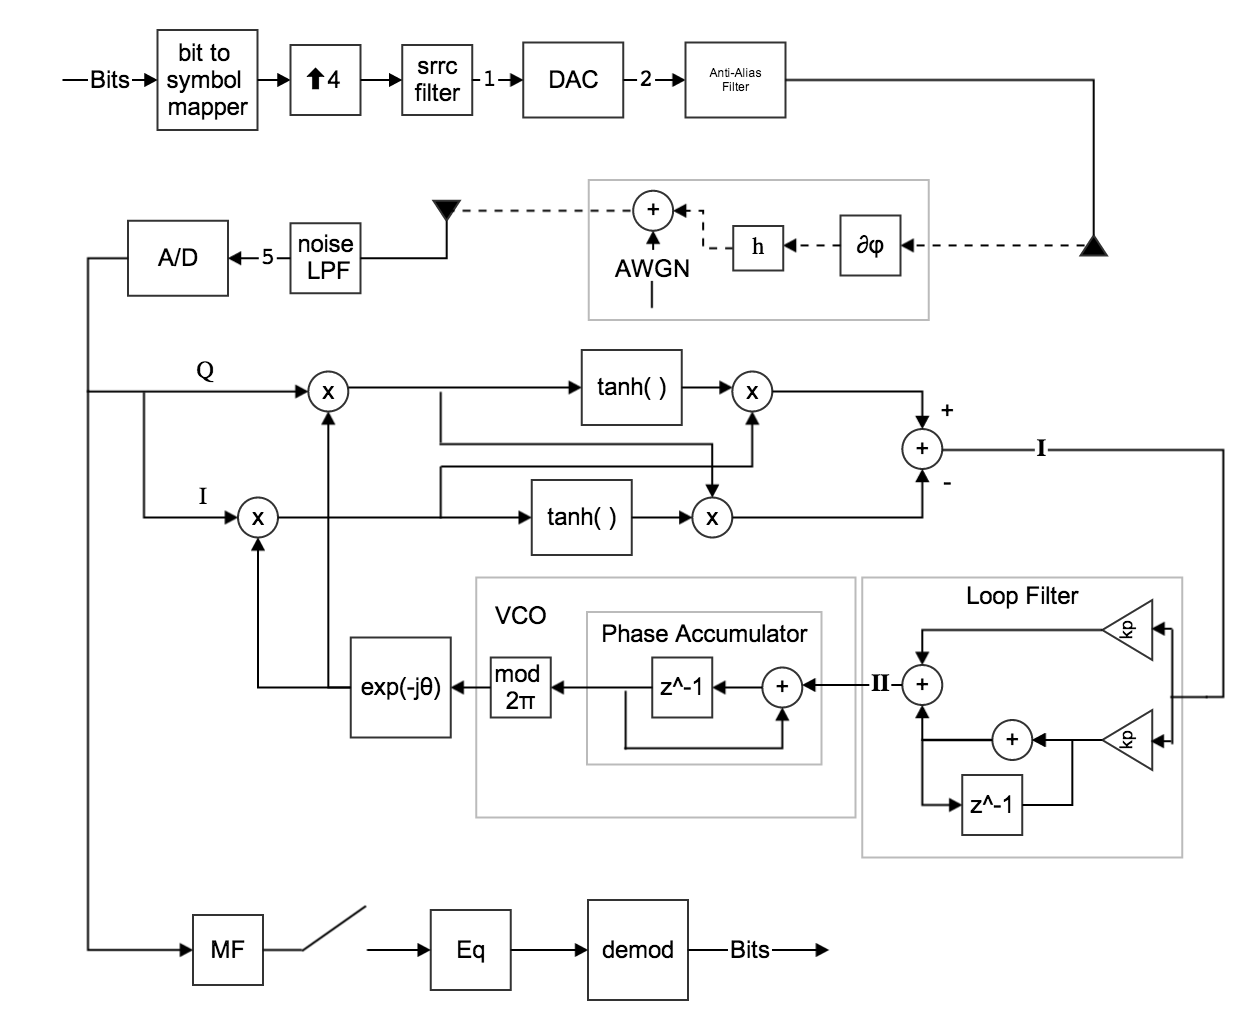
\includegraphics[width=\textwidth]{systemfinal.png}
\caption{Full System Block Diagram\label{fig:system}}
\end{figure}


Some vital information about the system parameters are listed below and each of the blocks seen on the figure are explained in detail in the following sections:
\begin{itemize}
\item Roll-off factor = 0.75
\item Sampling Period = 10ns
\item Equalizer = ZF
\item Number of taps =
\item Cut-off frequency = 
\item Modulation scheme = QPSK/16QAM
\end{itemize}

\subsection{Bit Generation}
\label{sec:bits}
 To start with, a random bit generator was used to output a stream of data (Appendix ~\ref{app:random_bit_generator}). In this generator we used MATLAB psuedorandom generating functions to ensure the information would be as well distributed as possible. To further ensure the modeling was fair, the number of bits generated was set to 48000. 
\subsection{Modulation}
\label{sec:modulation}
The data stream was then passed into a bit-to-symbol mapper, transformed differently based on the modulation scheme  (Appendix~\ref{app:bittosym}).  Two  modulation schemes were used, including:
\begin{itemize}
\item Quadrature Phase Shift Keying [QPSK] which maps bits to symbols  as shown in the following constellation plot:

	\begin{figure}[H]
	\centering
	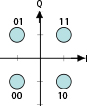
\includegraphics[width=.2\textwidth]{QPSK.jpg}
	\caption{QPSK constellation plot showing bit to 		symbol mapping}
	\end{figure}

\item 16 - Quadrature Amplitude Modulation [16-QAM] which maps bits to symbols as shown in the following constellation plot:

	\begin{figure}[H]
	\centering
	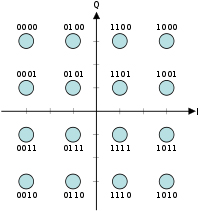
\includegraphics[width=.3\textwidth]	{16QAM.jpg}
	\caption{16-QAM constellation plot showing bit to 	symbol mapping}
	\end{figure}

\end{itemize}

as shown in Appendix ~\ref{app:qpsk_mod}, ~\ref{app:qam_16_mod}.

It should be noted that oth of the modulation schemes use Grey Coding which makes sure there is only one bit difference between neighbouring symbols. This greatly decreases the bit error rate as we are forcing only one bit to be different if a neighbouring symbol is demodulated instead of the correct one. 

\subsection{Oversampling}
\label{sec:oversample}
In order to manipulate the signal without loss, the data was oversampled by four [Appendix~\ref{app:impulse_train}].  To do so, the code block zero pads the input so that an impulse train is passed along.  The sampling rate, because of this, exceeded the Nyquist sampling rule but allowed us to have some extra leeway to work with.   

\subsection{Pulse Shaping}
\label{sec:srrc}
To approximate a real system, the signal is put through a square root raised cosine filter in order to represent symbols as pulses that can be transferred over a channel. This filter has the following impulse response:

 \[
 h(t) = \begin{dcases*}
        1-\beta+4\frac{\beta}{\pi} &  $t = 0$\\ \\        
        \frac{\beta}{\sqrt{2}}\left[\left(1+\frac{2}{\pi}\right)\sin\left(\frac{\pi}{4\beta}\right)+\left(1-\frac{2}{\pi}\right)\cos\left(\frac{\pi}{4\beta}\right)\right] & $t=\pm \frac{T_s}{4\beta}$ \\ \\
        \frac{\sin\left[\pi\frac{t}{Ts}\left(1-\beta\right)\right]+4\beta\frac{t}{Ts}\cos\left[\pi\frac{t}{Ts}\left(1+\beta\right)\right]}{\pi\frac{t}{Ts}\left[1-\left(4\beta\frac{t}{Ts}\right)^2\right]} & $otherwise$ \\
        \end{dcases*}
\]

as implemented in Appendix ~\ref{app:sqrt_raised_cosine}.  \\

One can question why another pulse shape, such rectangular function, isn't used in the project. The answer is, because square root raised cosine pulse is a common tool to combat inter symbol interference [Section~\ref{sec:ISIbackground}].  This is caused by the fact that it is a Nyquist pulse with a flat spectrum. In other words because the raised cosine has zero impulse response at all integer multiples of its period, correct sampling can perfectly reconstruct the signal without having delayed symbol muddle the waveform. 

\subsection{Digital-to-Analog Conversion}
\label{sec:da}

The output of this shaping filter (\#1 in Figure ~\ref{fig:system}) is fed into a Digital-to-Analog Converter (DAC).  A DAC takes the digital samples and zero-order holds them at a constant voltage, creating an analog signal. At this point, the signal is assumed to be sent through physical components. The demonstration of this conversion can be seen in Figure ~\ref{fig:dtoa} \\

The implementation of this block can is shown in Appendix ~\ref{app:da}, ~\ref{app:zero}.

\subsection{Anti-Aliasing Reconstruction Filter}
\label{sec:reconstruction}
After the analog to digital conversion, a reconstruction filter (also called an anti-aliasing filter) bandlimits the analog waveform output from the DAC (\#2 in Figure ~\ref{fig:system}).  The high frequency content contained in the stair-case digital signal is undesirable since it can create aliasing of wrongfully high frequency waves. To avoid this, the Low Pass Filter is used for the reconstruction.  Ours is modeled as a Butterworth filter, or a maximally flat magnitude filter.  The aim of the filter is to have uniformly flat passband frequency response and roll to zero in the stopband.  As with all filters, the cutoff frequency parameter sets the bands and the order of the filter determines the roll-off of the frequency response in the stopband.  We used a fourth order Butterworth so that the roll-off was $80 \mathtt{\frac{dB}{dec}}$.  We set the cutoff frequency approx. to $\frac{\pi}{20}$ $\mathtt{Hz}$ at the TX part. The interior workings of the filter are not pertinent to this project, so the code in Appendix~\ref{app:butterworth} uses built-in MATLAB functions. Furthermore the issues and challenges caused by bilinear transformation of an analog filter to digital filter and TX cut-off frequency sensitivity are addressed in Section ~\ref{sec:issues}. \\

At this point (\#3 in Figure ~\ref{fig:system}), the waveform gets be transmitted through the medium. \\

A demonstration of the output of this filter can be seen in Figure ~\ref{fig:dtoa}.

	\begin{figure}[H]
	\centering
	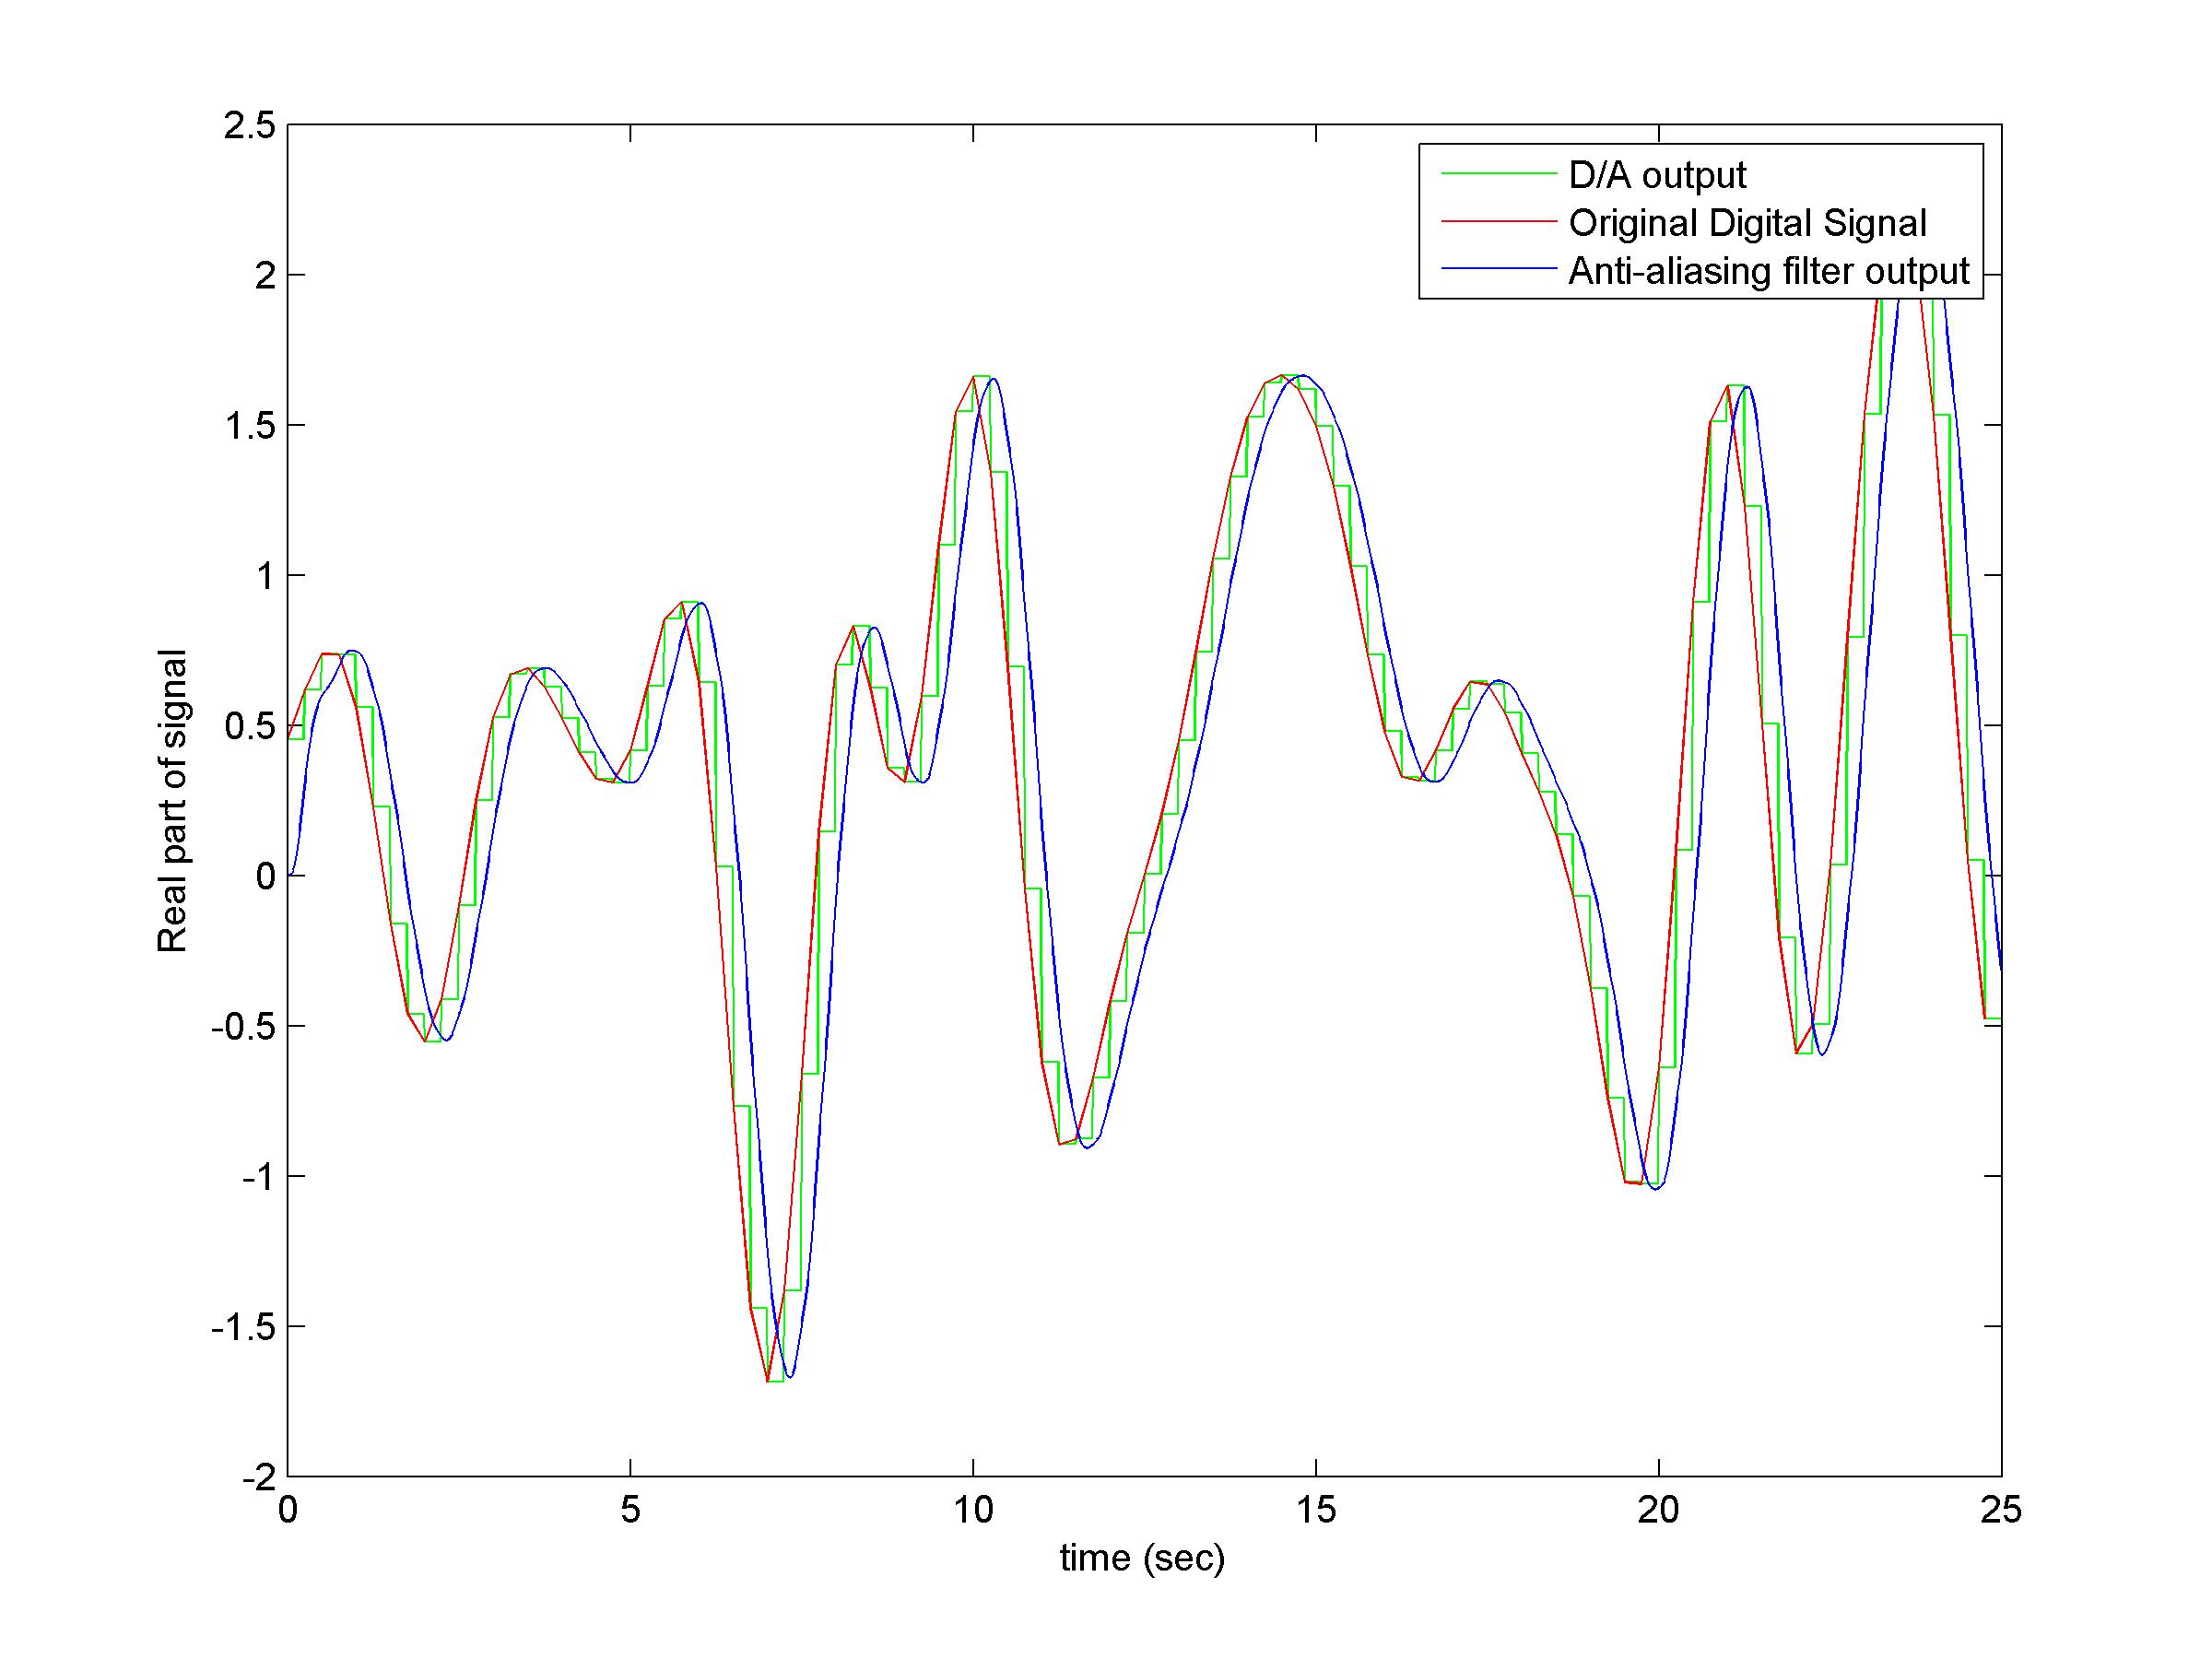
\includegraphics[width=\textwidth]	{DtoA.jpg}
	\caption{The original digital signal and the outputs of D/A converter and anti-aliasing filter at SNR=100dB for the first 100 symbols (QPSK modulation)\label{fig:dtoa}}
	\end{figure}

\subsection{Channel Medium}
After processing the data at the TX end of the system, it is sent through a bandlimited channel which is modelled to produce a phase error, white gaussian noise. 

\label{sec:channel}
\subsubsection{Phase Error}
\label{sec:phaseError}
To enhance the realism of the model, non-coherent error was included in the transmission. The $\delta\phi$ block represents a block that introduces frequency offset on the carrier.  The effect of this is to blur the symbol constellations.  \\

The new block was modeled by introducing a first order phase term.  Recall, phase is related to frequency by Equation ~\ref{eq:phaseToFreq}.

\begin{equation}
\label{eq:phaseToFreq}
f(t) = \frac{1}{2 \pi} \phi^\prime(t)
\end{equation}

Appendix ~\ref{app:freq} shows how this was implemented in the simulations.  We used a frequency offset of $100 \mathtt{kHz}$.  



\subsubsection{Channel Gain}
\label{sec:channelFilter}
We  have the following bandlimited channel response installed in our system model:
 $$h(t) = 0.1\delta(t + 100 \mathtt{ns}) + 0.8\delta(t -40 \mathtt{ns}) + 0.95\delta(t - 30 \mathtt{ns}) + 0.7\delta(t - 100 \mathtt{ns}) - 0.35\delta(t - 170 \mathtt{ns})  $$
 
This has to be converted into vector from in order to process in MATLAB. Thus the following calculation is made: 
 
 $$h(t) = 0.1\delta(t + 100 \frac{\mathtt{ns}}{T_s}) + 0.8\delta(t -40 \frac{\mathtt{ns}}{T_s}) + 0.95\delta(t - 30 \frac{\mathtt{ns}}{T_s}) + 0.7\delta(t - 100 \frac{\mathtt{ns}}{T_s}) - 0.35\delta(t - 170 \frac{\mathtt{ns}}{T_s})  $$
 
Although this channel introduces significant ISI, we have perfect knowledge of the channel, so handling the interference is not difficult. \\

The implementation of the bandlimited channel is shown in Appendix ~\ref{app:bandlimited}.

\subsubsection{Noise}
\label{sec:awgn}
The channel additionally has a source of Additive White Gaussian Noise (AWGN) as implemented in Appendix~\ref{app:awgn_channel}. The variance of this channel noise is determined by the SNR values picked at the beginning of each simulation. We can relate the two by the following:

$$\sigma^2 = \frac{S}{10^{SNR/10}}$$
where S is the average signal power of the chosen modulation scheme.  This is then the end of the channel model (\#4 in Figure ~\ref{fig:system}). \\

We could have had this noise be colored by the channel itself, but could just have easily used a whitening filter to flatten the frequency response back to Gaussian.  Such a complication could be added in future models.  

\subsection{Noise Limiting Filter}
\label{sec:noiseLPF}
An anti-aliasing low-pass filter constrains, or band limits, the channel-filtered waveform (\#5 in Figure ~\ref{fig:system}).  In this setting, the LPF protects against aliasing of high frequency content being recorded at the lower frequency.  We use the same Butterworth filter (implemented in Appendix ~\ref{app:butterworth} ) to accomplish this function set the cut-off frequency to approx. $\frac{\pi}{50}$ $\mathtt{Hz}$ at the RX. The output of this filter is demonstrated in Figure ~\ref{fig:atod}. Furthermore the issues and challenges caused by bilinear transformation of an analog filter to digital filter and RX cut-off frequency sensitivity are addressed in Section ~\ref{sec:issues}.

\subsection{Analog-To-Digital Converter}
\label{sec:adc}
To bring the analog waveform back to the digital world, an Analog-to-Digital converter is used [Appendix~\ref{app:ad}].  From here (\#6 in Figure ~\ref{fig:system}) on out, the waveform is back in the digital domain for processing. \\

A demonstration of the output of this block can be seen in Figure ~\ref{fig:atod} and the issues and challenges caused by the sampling instances of the converter is addressed in Section ~\ref{sec:issues}.

	\begin{figure}[H]
	\centering
	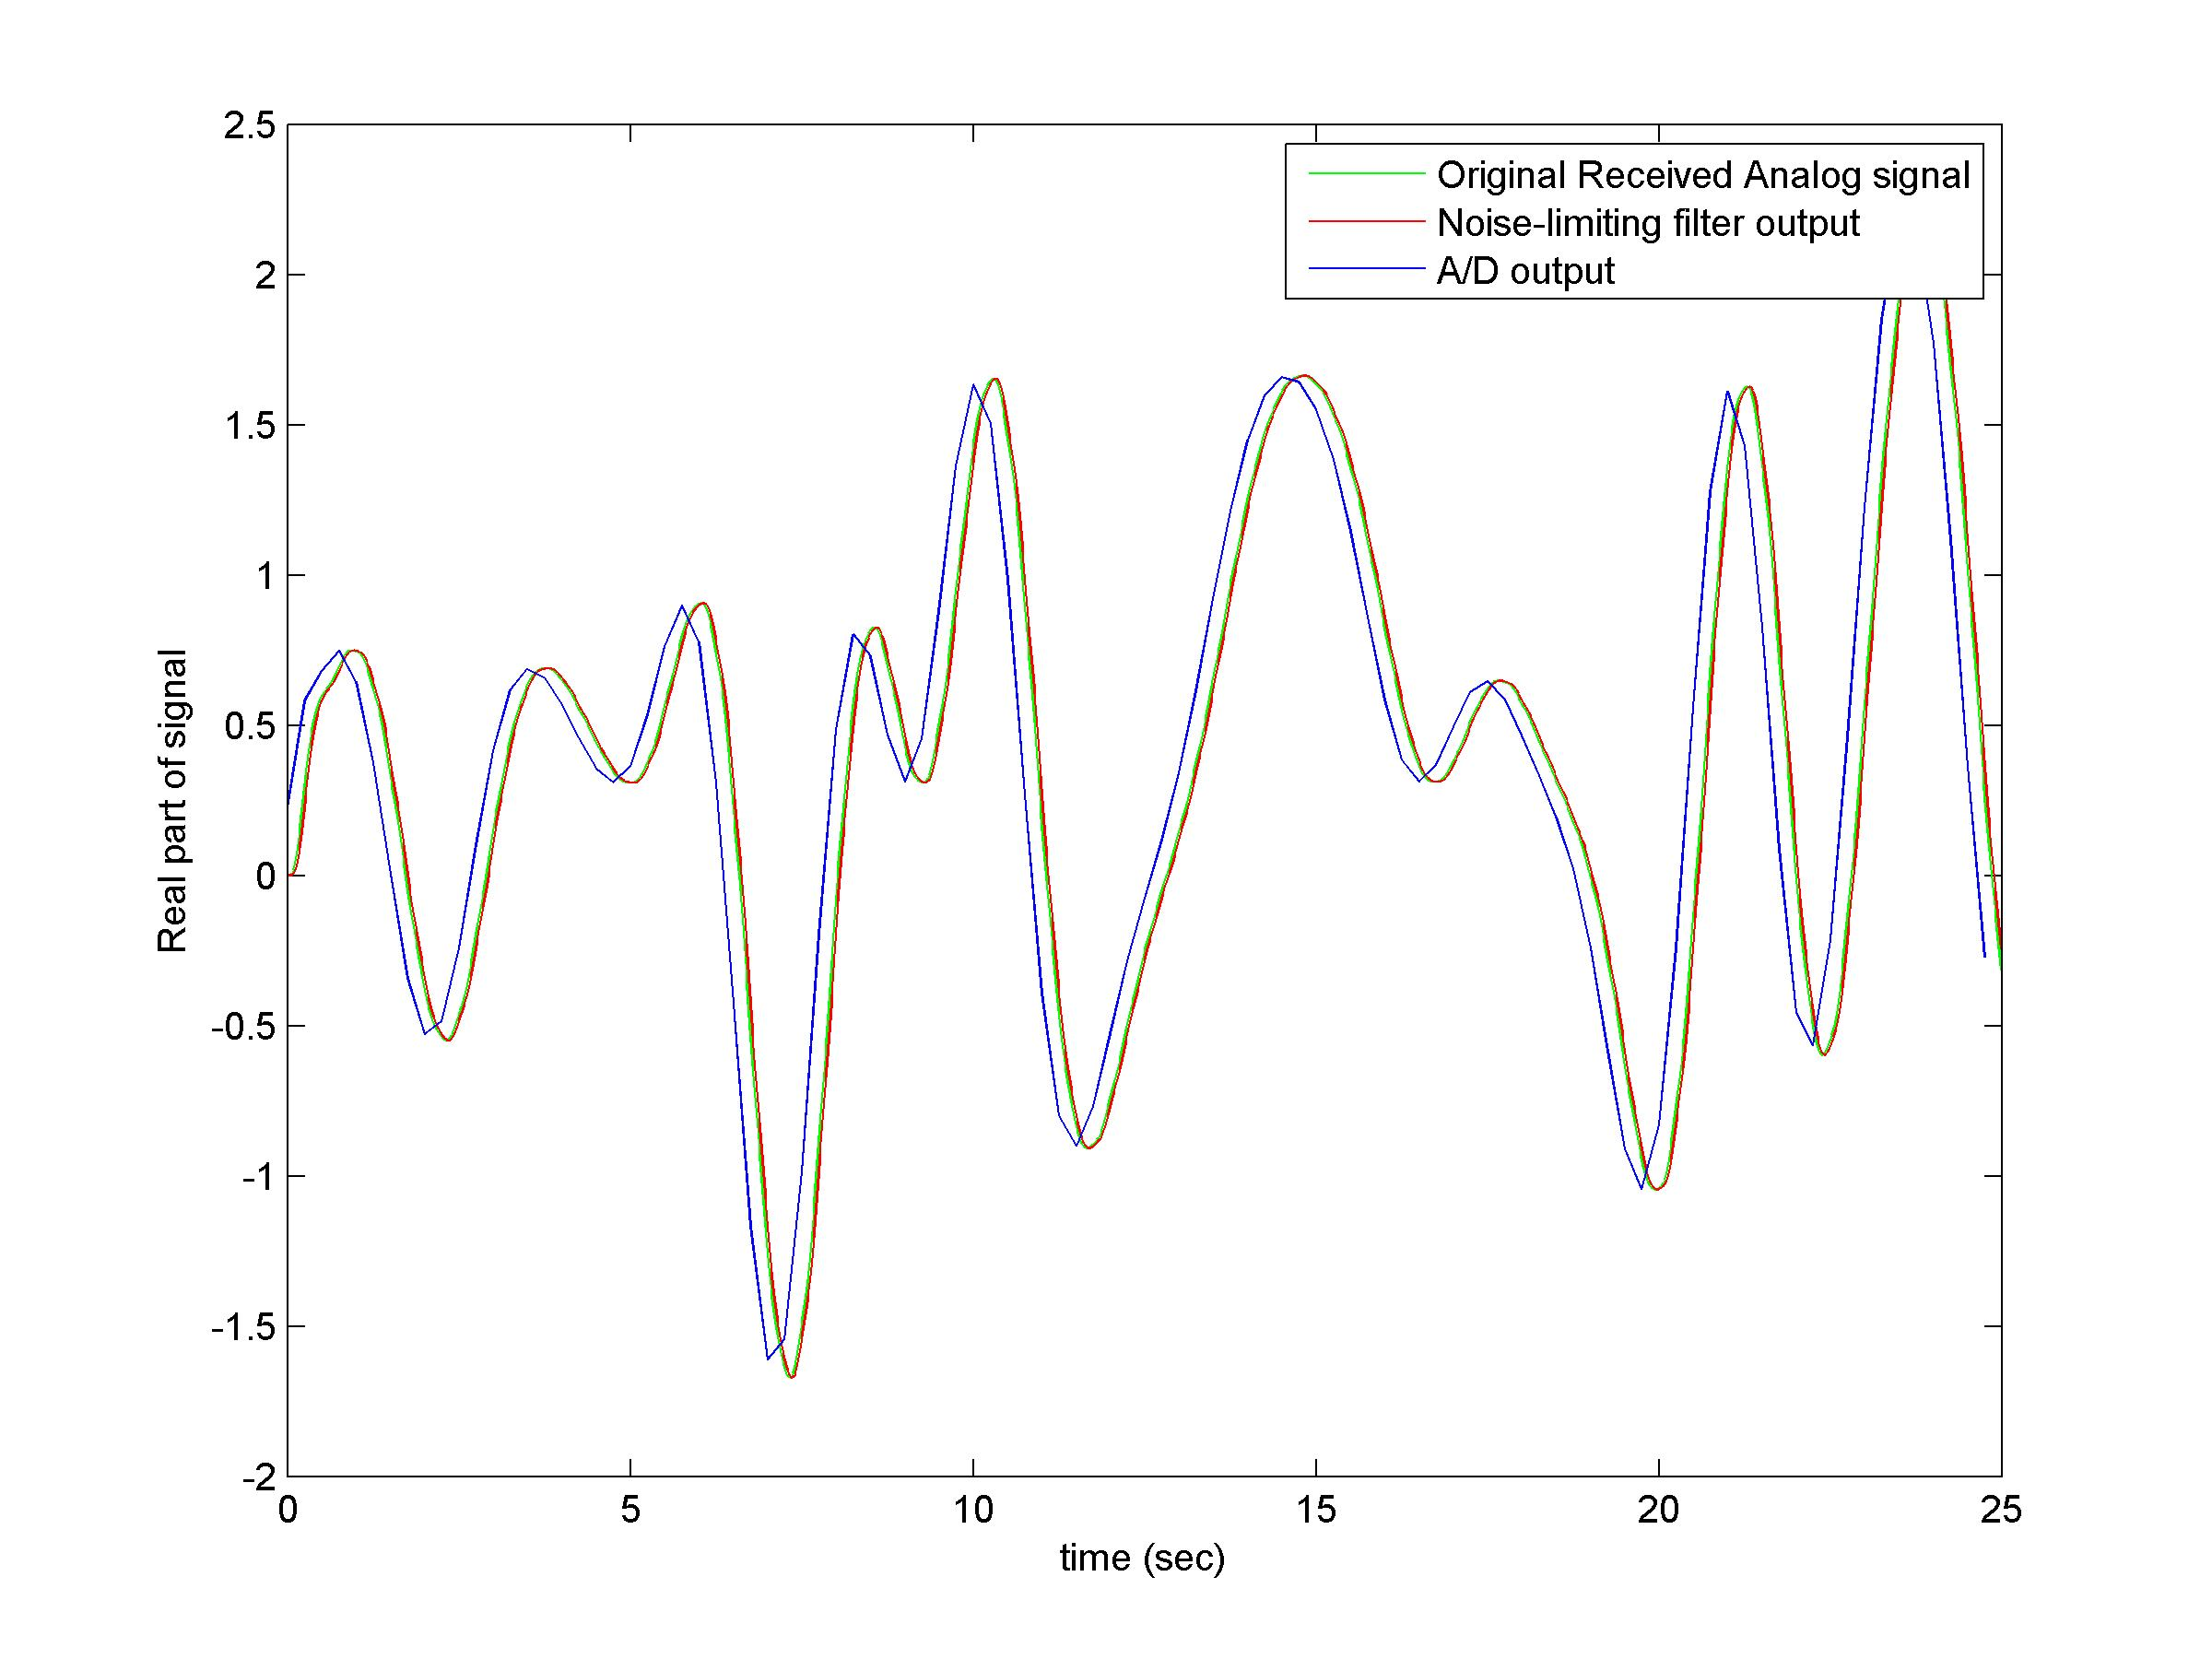
\includegraphics[width=\textwidth]	{AtoD.jpg}
	\caption{The original received analog signal and the outputs of A/D converter and noise-limiting filter at SNR=100dB for the first 100 symbols (QPSK modulation)\label{fig:atod}}
	\end{figure}


\subsection{Tracking Loop}
\label{sec:tracking}
The frequency offset  recovery is accomplished via a Costas loop (Feedback background is explained in explained in detail in Section ~\ref{sec:feedback}) whose implementation is given in Appendix ~\ref{eq:costas}. The I and Q component of the received signal (\#7i and \#7q in Figure ~\ref{fig:system}) are both sent through a $\tanh\left(\cdot\right)$ block in order to discern their sign.  This works because, for $k>>1$, $\text{sign}\left(x\right) \approx \tanh \left(x\right)$.  These $\pm1$ signals are multiplied by the opposite component signal.  The I component is then subtracted from the Q component, creating a phase error metric [\ref{eq:costas}].  This is labeled in Figure~\ref{fig:system} as \#8. 

\begin{align}
  \label{eq:costas}
  S_{\rom{1}} &= \left[I\left(t\right)\sin\left(\phi_e\right)+Q\left(t\right)\cos\left(\phi_e\right)\right]\text{sign}\left(I\left(t\right)\cos\left(\phi_e\right)- Q\left(t\right)\sin\left(\phi_e\right)\right)\nonumber \\
  &\qquad {} - \left[I\left(t\right)\cos\left(\phi_e\right)-Q\left(t\right)\sin\left(\phi_e\right)\right]\text{sign}\left(I\left(t\right)\sin\left(\phi_e\right)+Q\left(t\right)\cos\left(\phi_e\right)\right)
  \end{align}

This value is run into the loop filter, the first integrater in the feedback leg of the loop, and then through the VCO, the second integrator.
  
\begin{align}
\label{eq:vco}
\phi_{\text{out}} &= \int \! k_{VCO}V_{in} \mathrm{d}t
\end{align}
A VCO is a device with output oscillation which is varied by the voltage level of the input.  The transfer function, relating the input to the output, for this block is shown in Equation~\ref{eq:vco}. The integral action can help eliminate phase error. To implement a VCO in simulation, a phase accumulator does the integration action and then, to keep the result in the correct domain, the result is put through a modulo $2\pi$ block. \\

Finally the I and Q components are recombined by a summer (\#10 in Figure ~\ref{fig:system}). \\

The crucial point in designing the feedback loop is finding the right coefficients for the loop filter which will provide a fast tracking of the frequency offset. This makes sure the loop reaches the steady state as fast as possible, thus less errors are seen in the output bits. \\

Another important issue we have to address is the challenges caused by using a phase tracker and two integrators to cancel out the frequency offset. This is discussed in Section ~\ref{sec:issues}.


\subsection{Matched Filter}
\label{sec:matched}
A matched filter is used for optimal detection of the transmitted signal. The same square root raised cosine pulse (as implemented in Appendix ~\ref{app:sqrt_raised_cosine}) is used to pick up the waveform (\#11 in Figure ~\ref{fig:system}).

\subsection{Sampler}
\label{sec:sample}
After the matched filter, the signal has to be sampled at BLAH $\mathtt{MHz}$.  We should keep in mind that the signal is oversampled by a factor of 4 in the TX end of the system. In other words the sampler has to pick one of the 4 oversampled points. Preferably the one with the highest value, meaning it is matched the best. Usually this is the value at the integer multiples of  $T_s$. \\

The implementation of this block is shown in Appendix~\ref{app:sampler}.

\subsection{ZF Equalizer}
\label{sec:equal}
The equalizer (necessary background for general architecture of equalizers is given in Section ~\ref{sec:ISIbackground}) we implemented was a Zero-Forcing (ZF) architecture as shown in ~\ref{app:zero}. To meet the goal of satisfying Condition~\ref{thm:zero}, the weight vector, $\mathbf{f}$, must perfectly negate all taps except the present-time one.  The present received symbol is a column within the $R$ matrix: $\mathbf{r}[i]$, often chosen to be the center one.  
$$ \mathbf{f}^{\ast}R = \mathbf{w}[i]^{\top} $$
Here, we used  $\mathbf{w} [i] \in \mathbb{R}^n$ to represent the i$^{th}$ Standard basis vector, or a column of zeros except in row $i$.  In this setting, we can find the tap weight vector to accomplish this by Equation~\ref{eq:zf}. 

\begin{equation}
\label{eq:zf} 
\mathbf{f}_{ZF} = R \left(R^{\ast}R \right)^{-1} \mathbf{w}
\end{equation}

\subsection{Demodulation}
\label{sec:demod}
After the equalization (\#11 in Figure ~\ref{fig:system}), the signal is ready to be mapped back into bits.  The demodulation in this block is the reverse of mapper used in the transmitter.  At this step, we are finally ready to evaluate how well the system worked.

\newpage

\section{Issues and Challenges}
\label{sec:issues}

\subsection{Bilinear Transformation}
An important issue we had to deal with, was the bilinear transform MATLAB uses to transform the analog Butterworth filter into the discrete domain. As shown in the figure below $tan(.)$ function is non-linear at higher frequencies and linear at frequencies close to 0:

\begin{figure}[H]
\centering
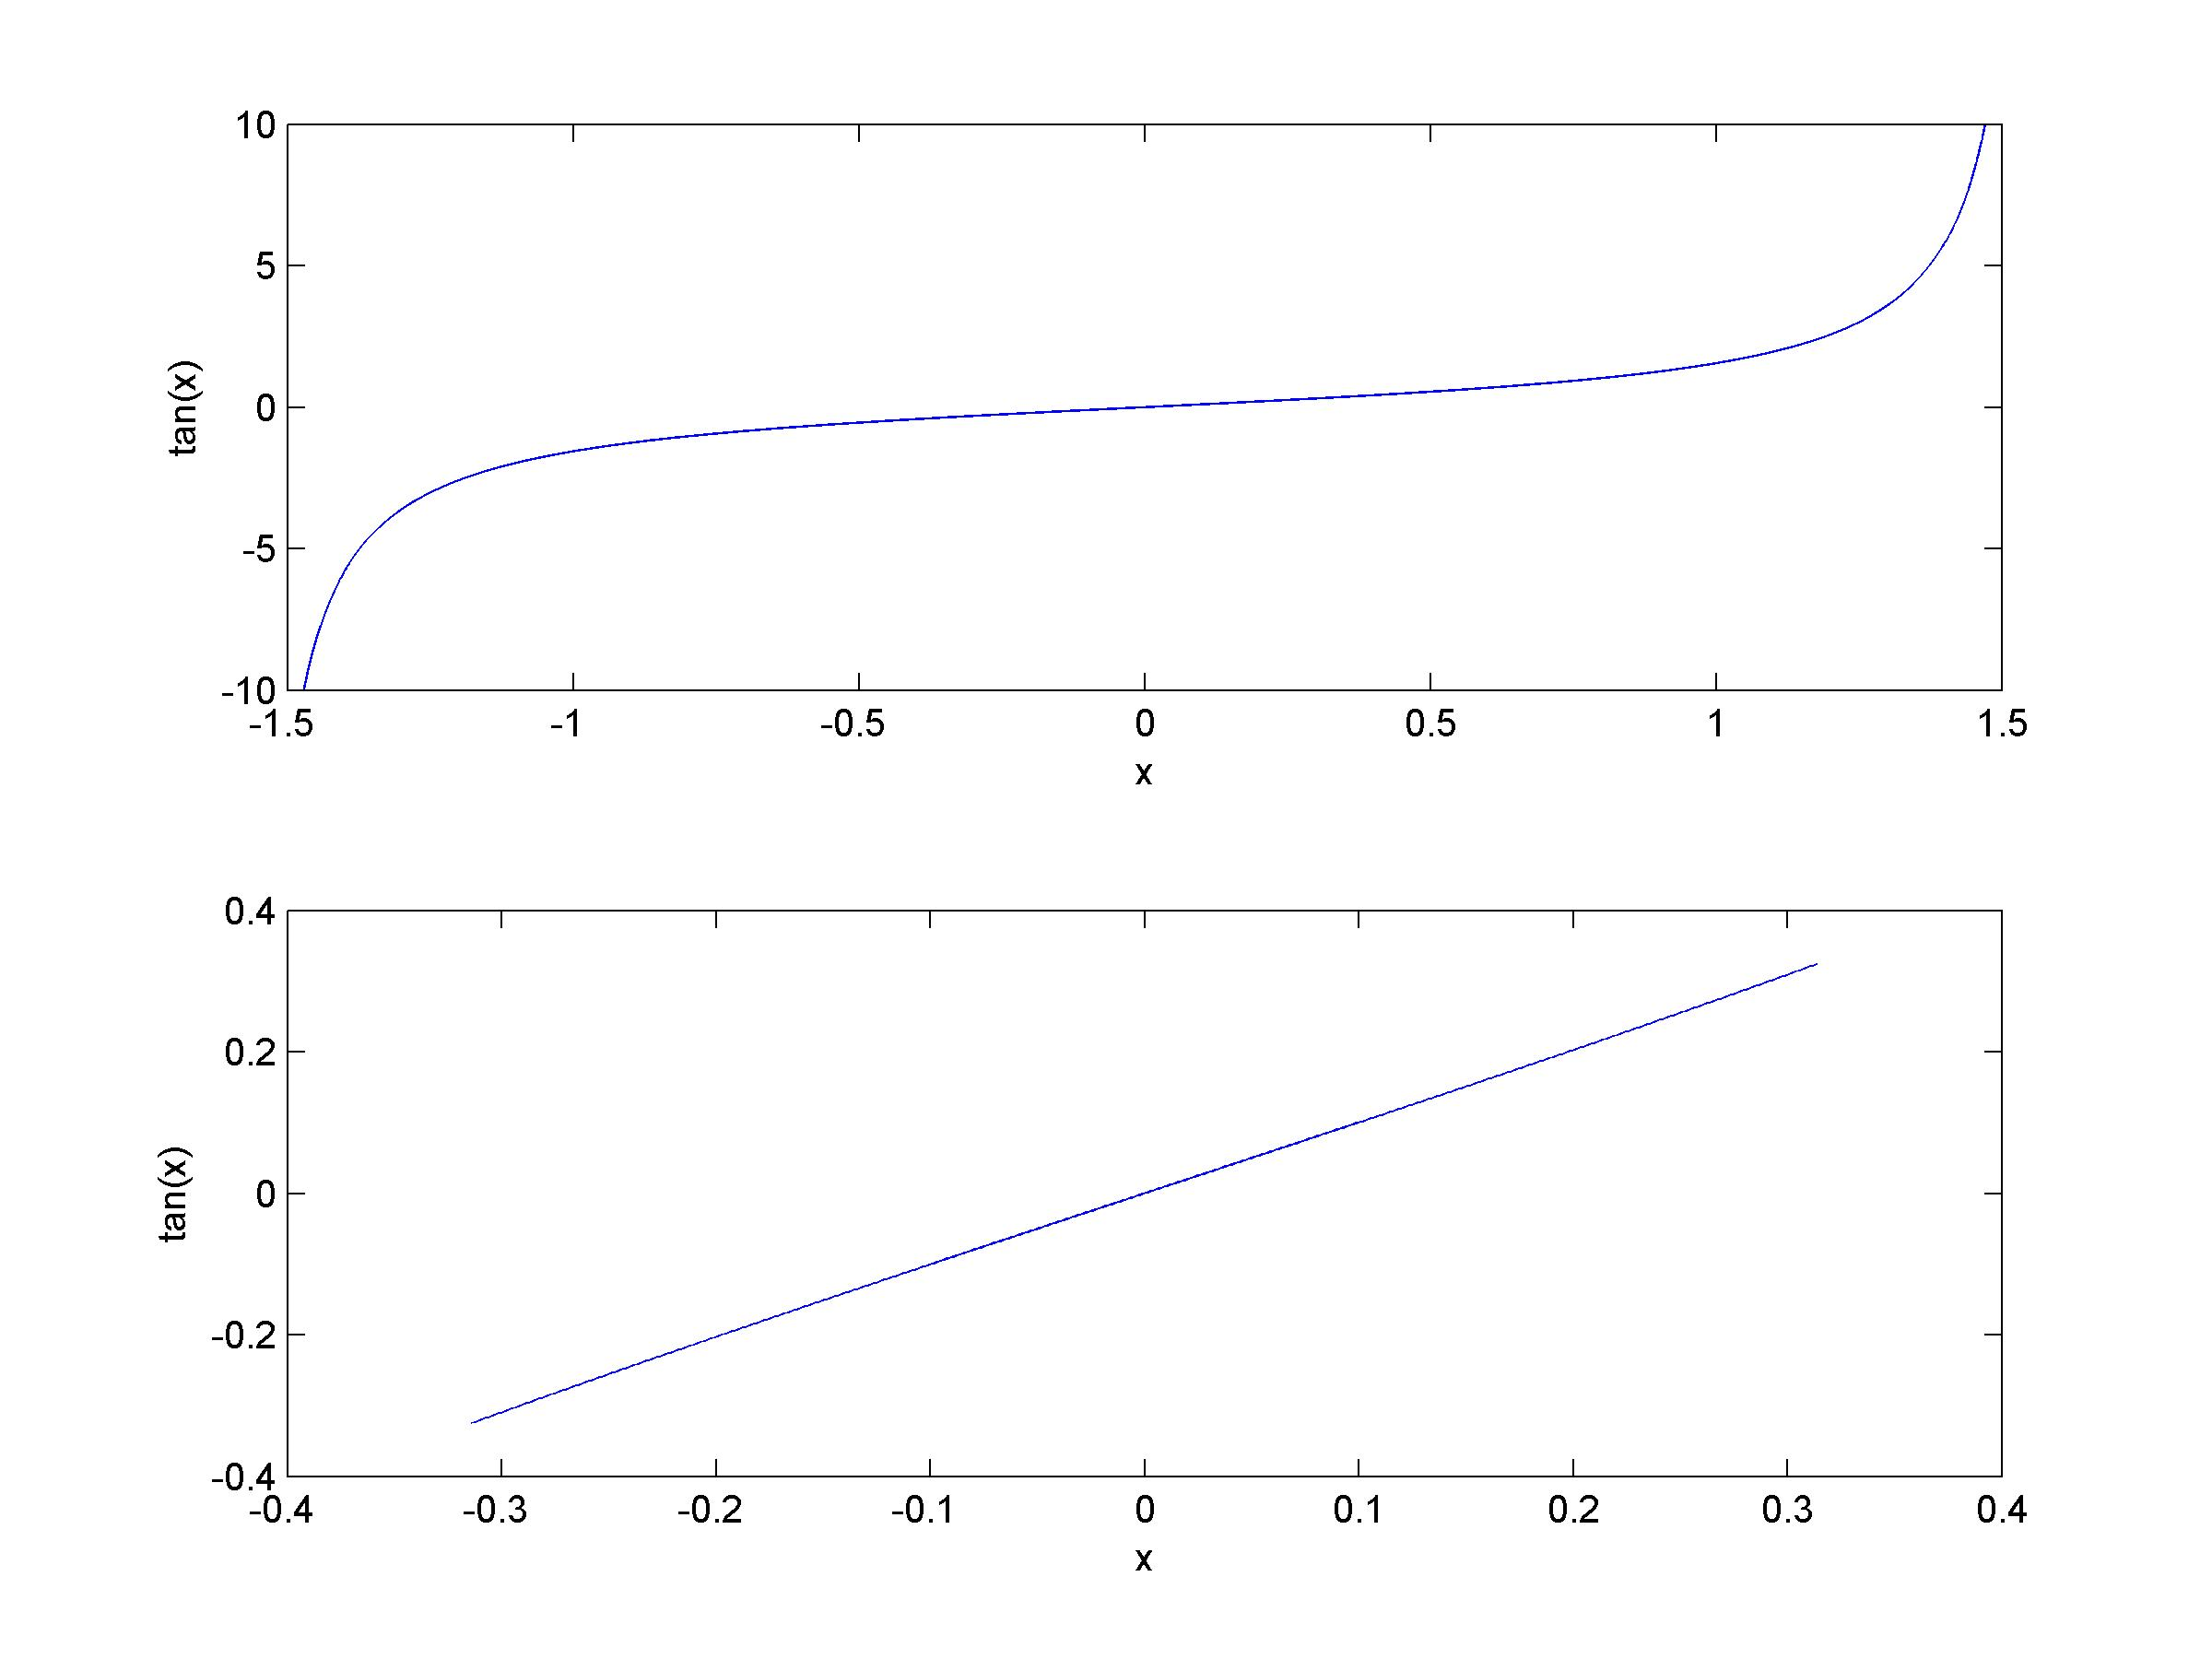
\includegraphics[width=0.7\textwidth]{tan_graph.jpg}
\caption{SER plot as a function of delay at the samplin g points of the A/D converter at SNR=20dB (QPSK modulation). \label{fig:delay}}
\end{figure} 

Thus in order to have cut-off frequencies at the linear regions (assumed to be linear around $\left[ -\pi/10,\pi/10 \right] $) of the $tan(.)$ function, the over sampling rate of the analog signal is set to 80 times more than the digital signal. \\

\subsection{TX Cut-off Frequency Sensitivity}
A sensitivity analysis is done for the cutoff frequency of the TX reconstruction filter. Recall, this filter is in place to bandlimit the DAC output so the high frequency content in the stairs does not create aliases in the lower, passband. The filter model is controlled by a normalized cutoff frequency, where zero and one are mapped to $\left(0,f_s\right)$.  As such, we expect that the cutoff frequency will not make much difference except if it is lower than $\pi/$(over sampling size of analog signal).  Even by choosing $f_c$ near $\pi/10$ (end of assumed linear region), all frequencies above the sampling frequency will be attenuated and the filter serves its purpose.  However, if $f_c$ gets too low, the information in the waveform may be lost. 
Figure~\ref{fig:freqTX} shows the sensitivity analysis of the anti-aliasing LPF normalized cutoff frequency. The graph confirms the expected behavior discussed above.

\begin{figure}[H]
\centering
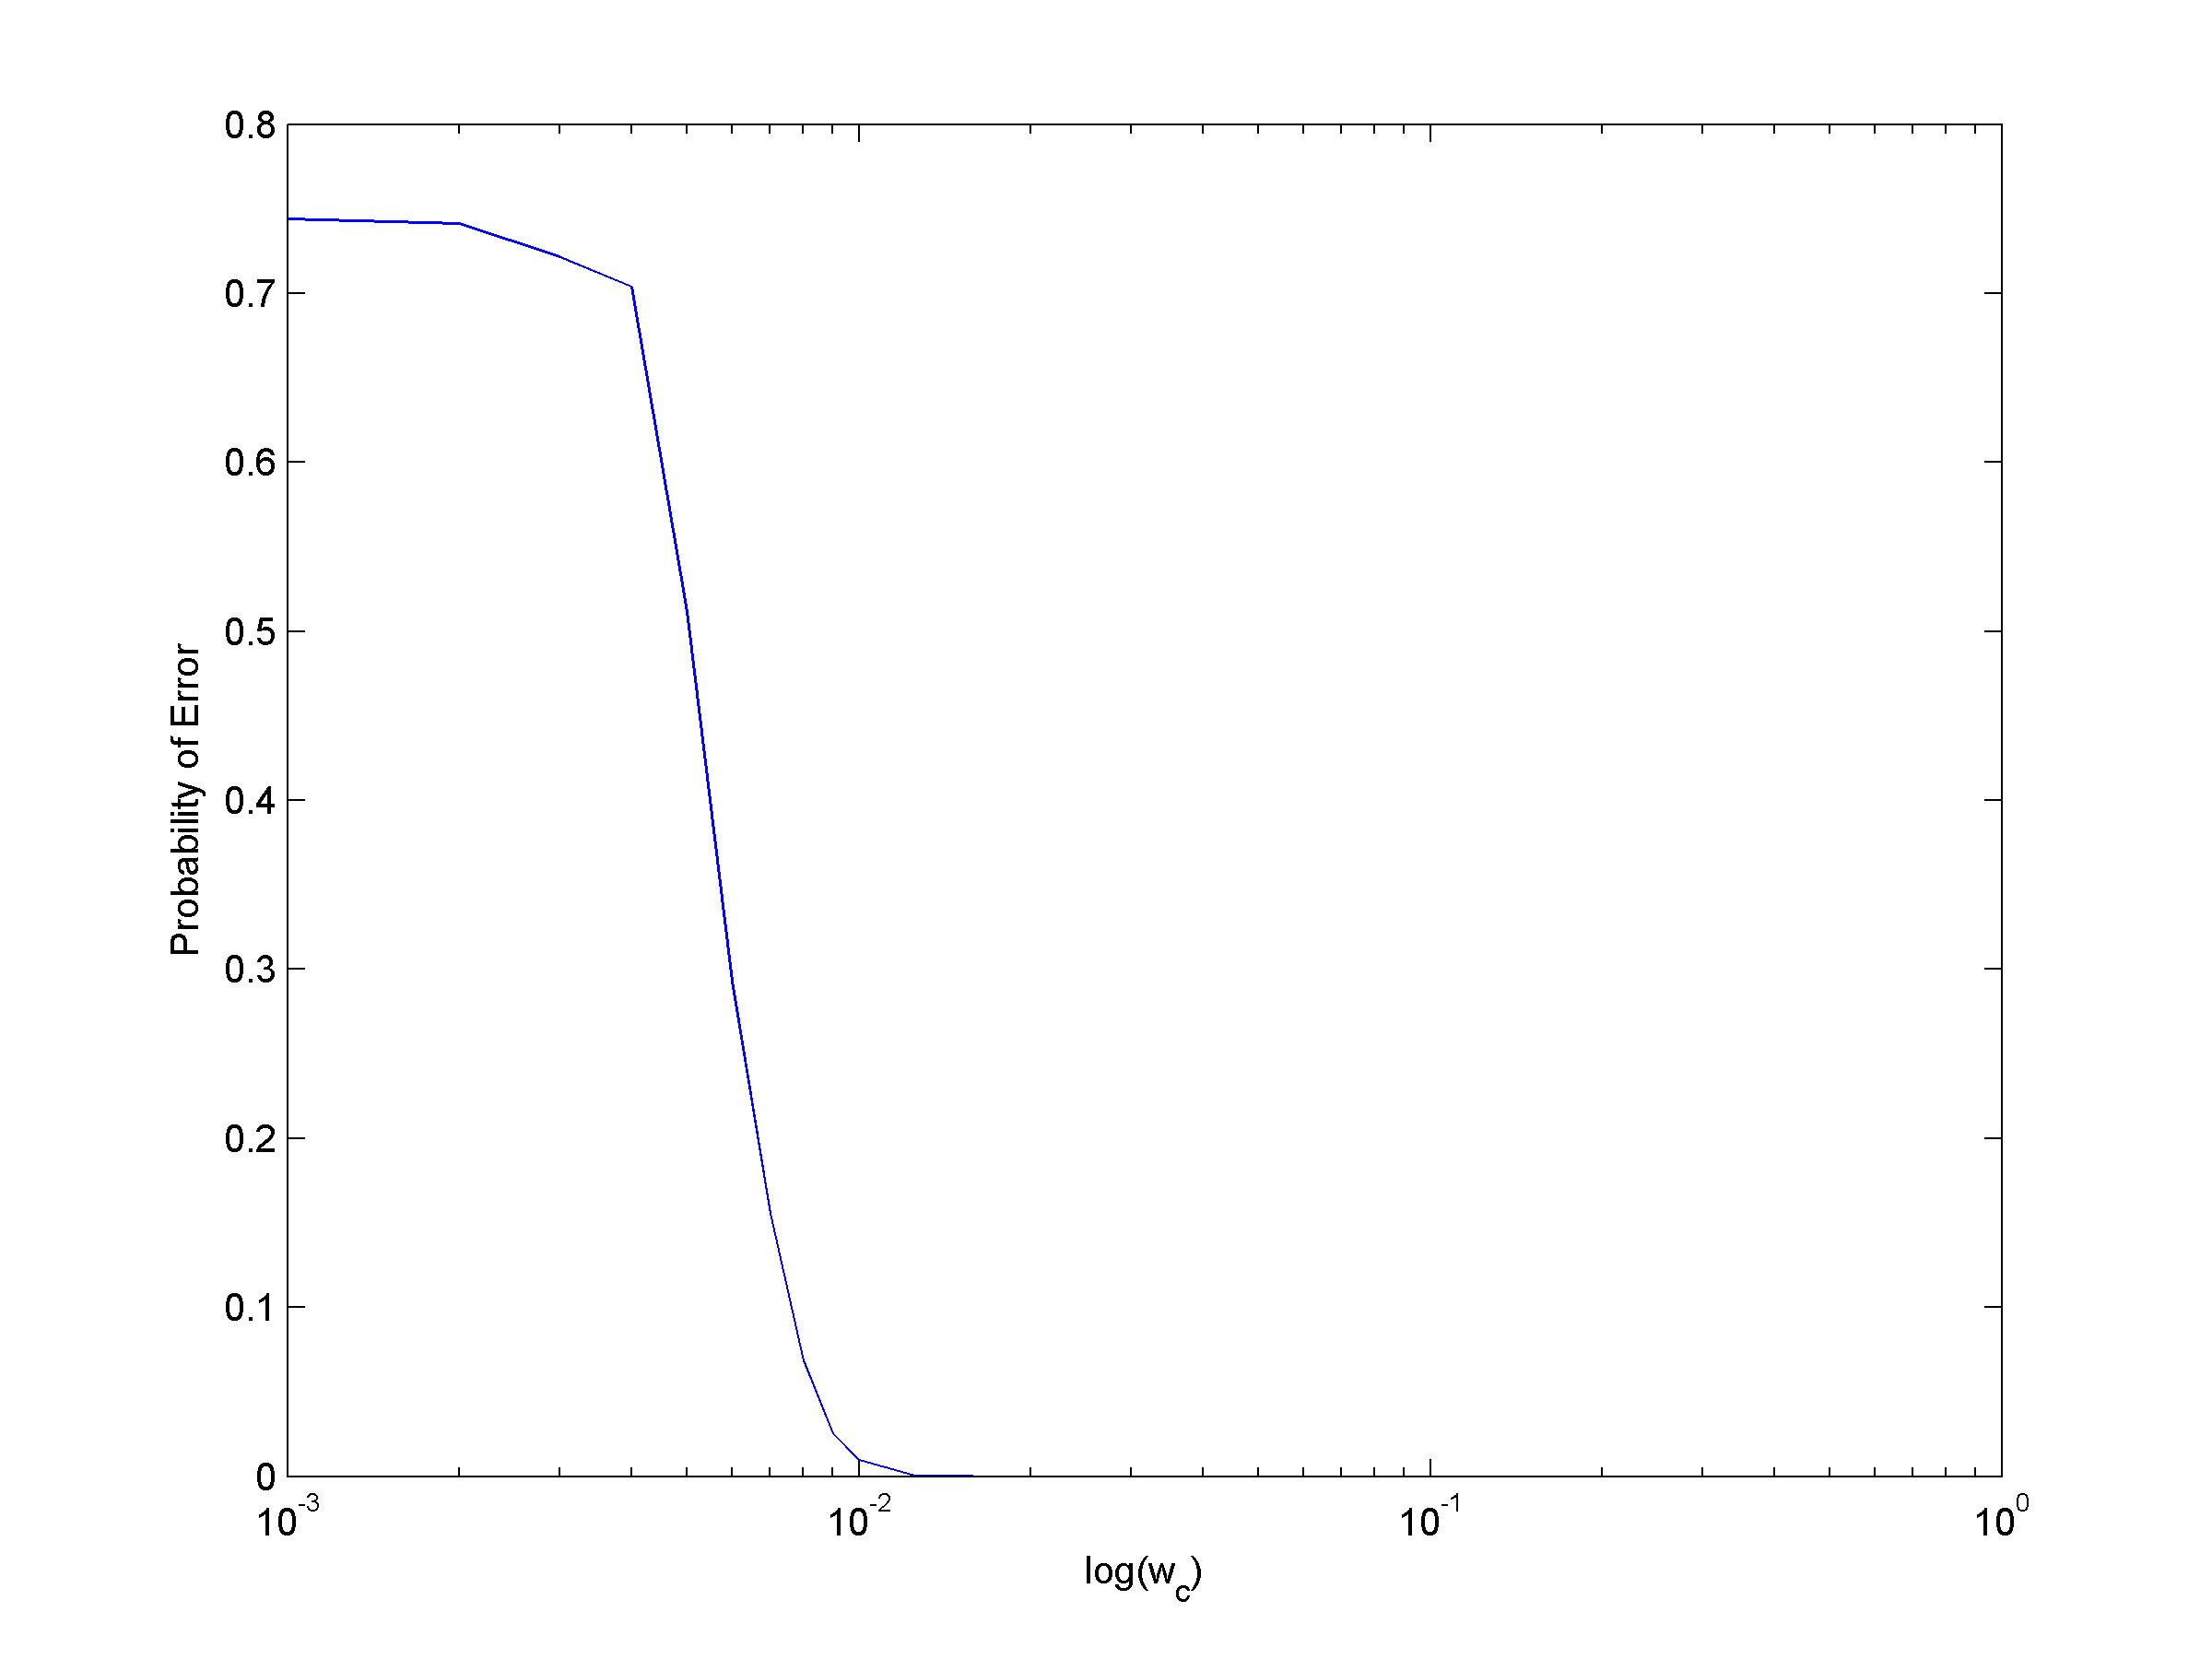
\includegraphics[width=0.6\textwidth]{freqTX.jpg}
\caption{SER plot as a function of cutoff frequency in the TX anti-aliasing Reconstruction filter at SNR=20dB (QPSK modulation). \label{fig:freqTX}}
\end{figure}

\subsection{RX Cut-off Frequency Sensitivity}

We performed a sensitivity analysis on the cutoff frequency in the RX noise-limiting filter. This filter was aimed to low pass filter the high frequency content from the noise and only allow the signal through. The same filter model was used with a lower cut-off frequency, so a similar trend was expected. Again at near zero cutoff, again we expect loss of data. But also this time, when the cut-off frequency is increased to the limits of the linear region we see an increase of the BER due to the fact that more noise is passing through the filter. Figure~\ref{fig:freqRX} shows the sensitivity analysis of the noise-limiting LPF normalized cutoff frequency. The graph confirms the expected behavior discussed above.

\begin{figure}[H]
\centering
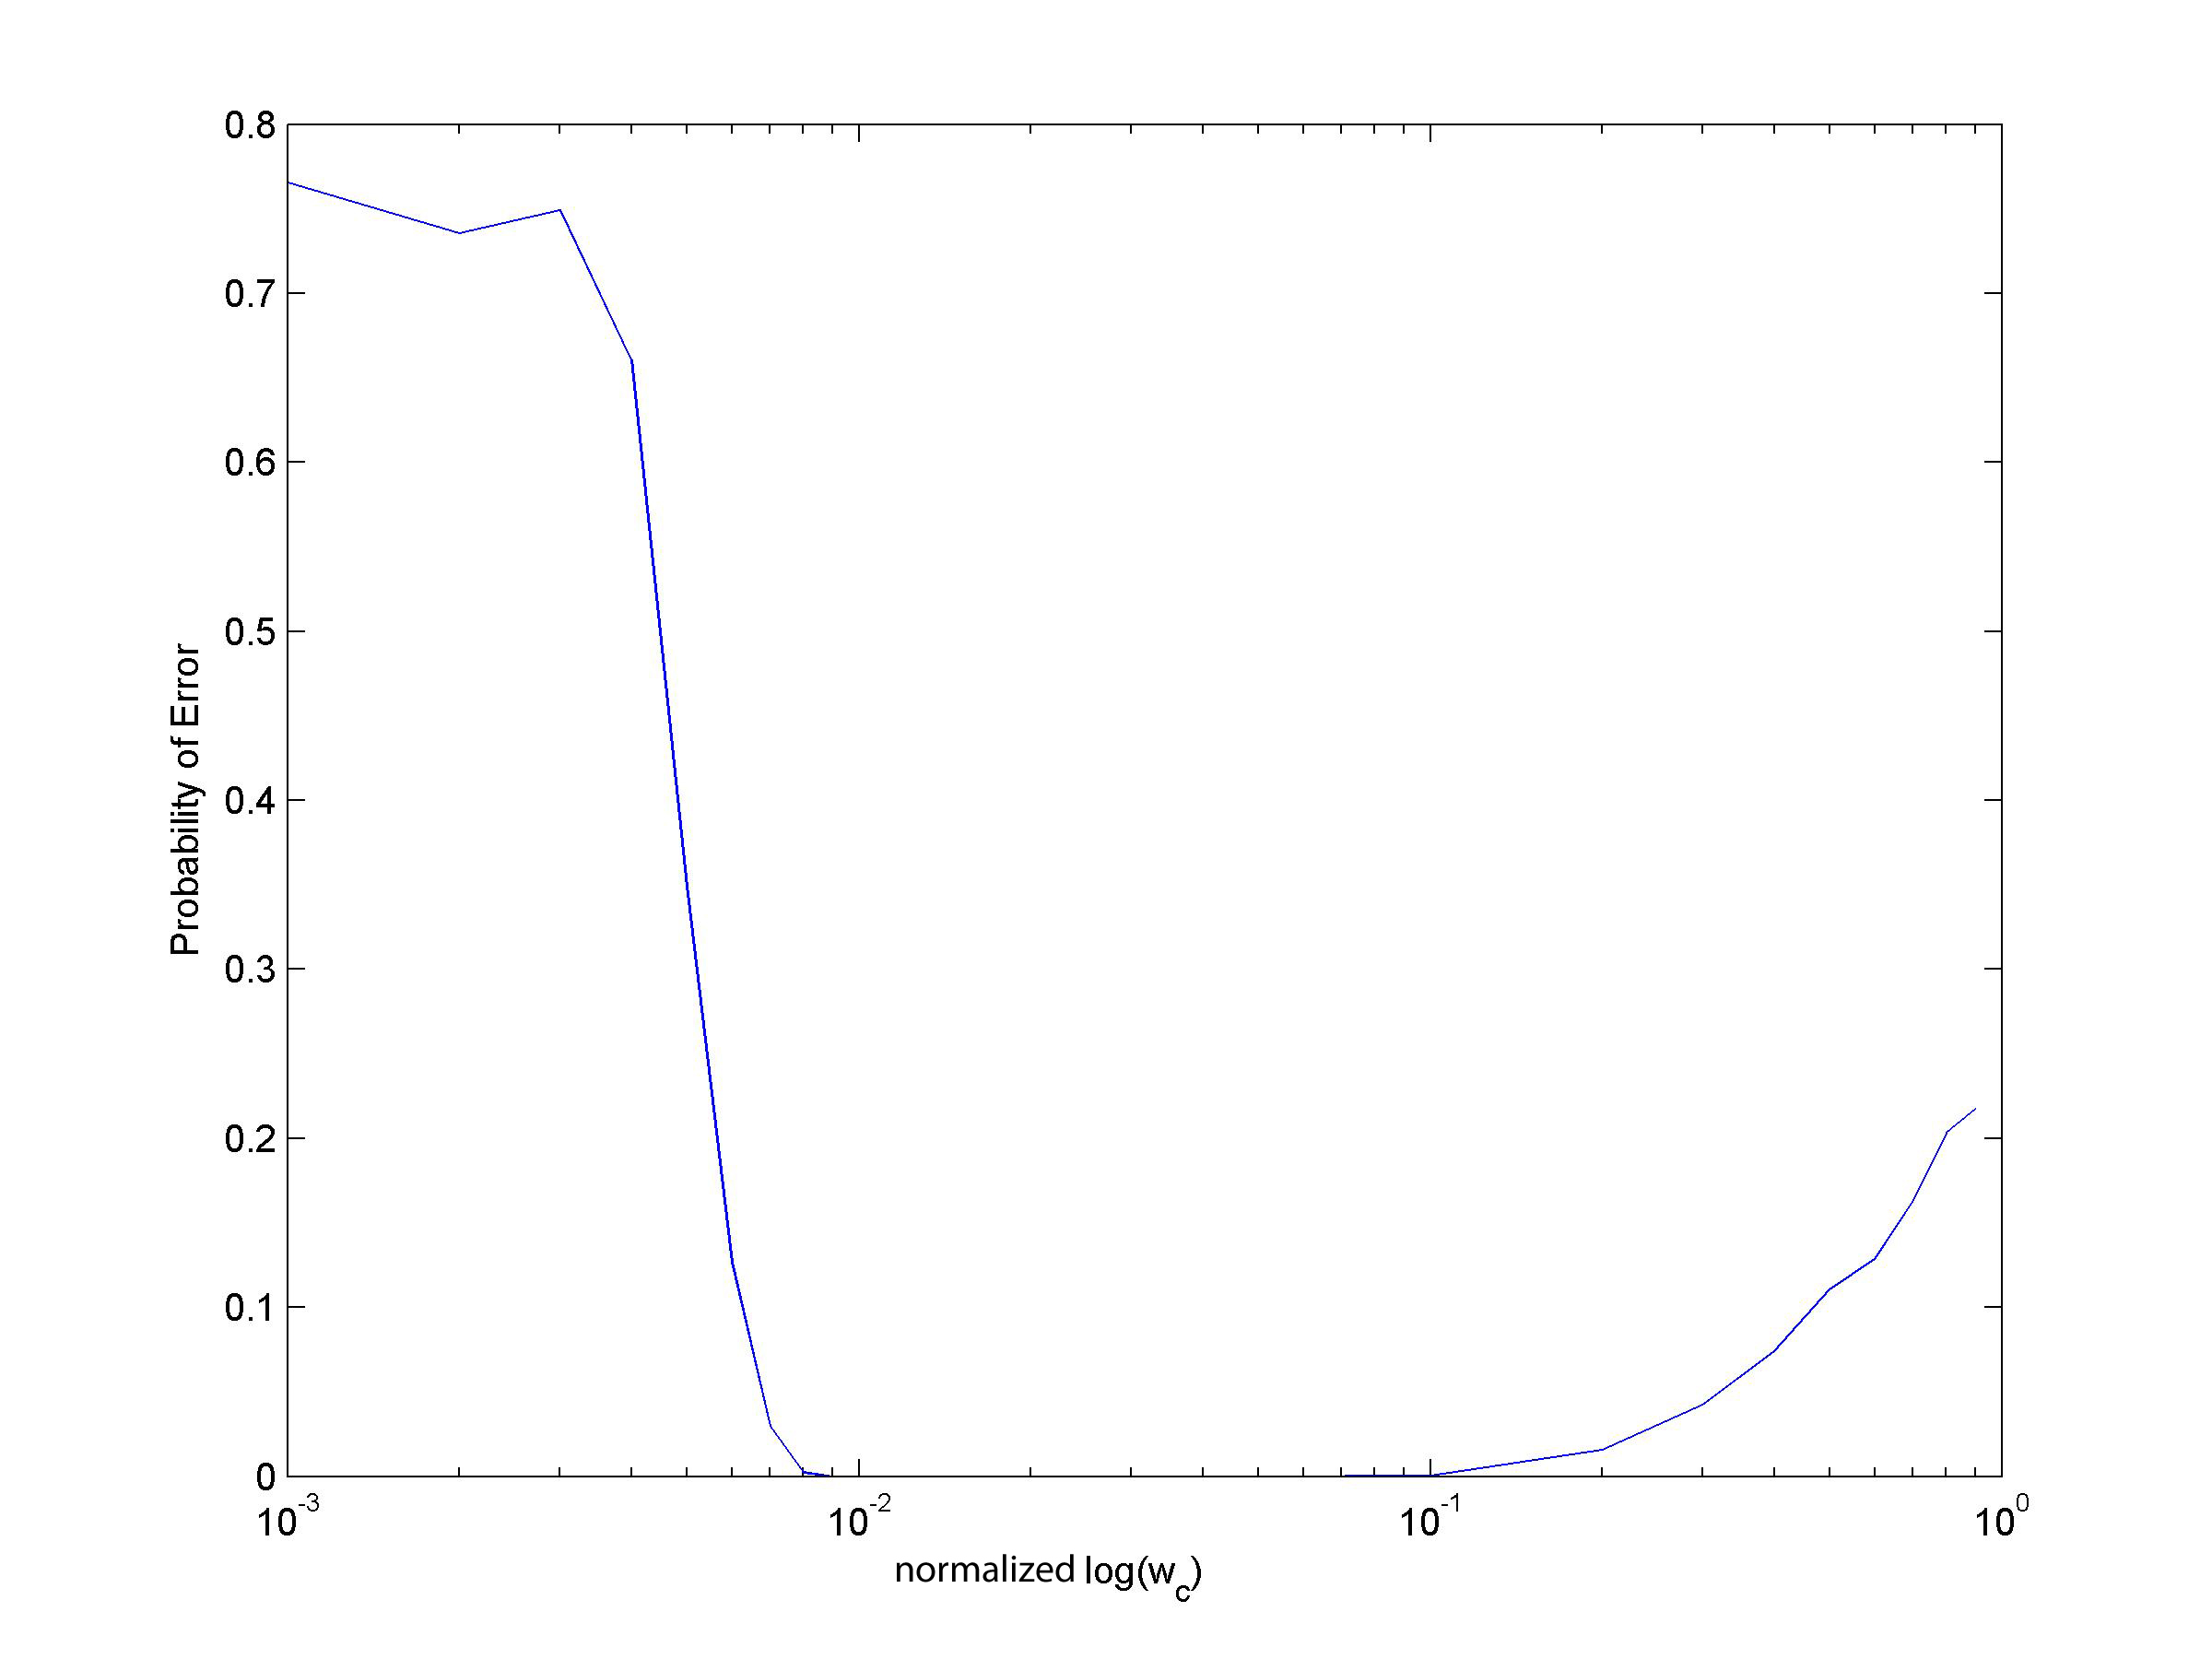
\includegraphics[width=0.6\textwidth]{freqRX.jpg}
\caption{SER plot as a function of cutoff frequency in the RX noise-limiting filter at SNR=20dB (QPSK modulation). \label{fig:freqRX}}
\end{figure}

\subsection{Sampling Delay Sensitivity}

The importance of sampling timing on the bit error rate is crucial due to the fact that we using low pass filters at both RX and TX  which delay the signals passing through them. From a sensitivity analysis of the delay through the system, the A/D will sample at varying degrees of synch. From such an experiment written in Appendix~\ref{app:delay}, when all other parameters like SNR and cutoff frequencies are kept equal to the optimal, we end up seeing the system works best at sampling delays 1 and 2. This is shown in Figure~\ref{fig:delay}.

\begin{figure}[H]
\centering
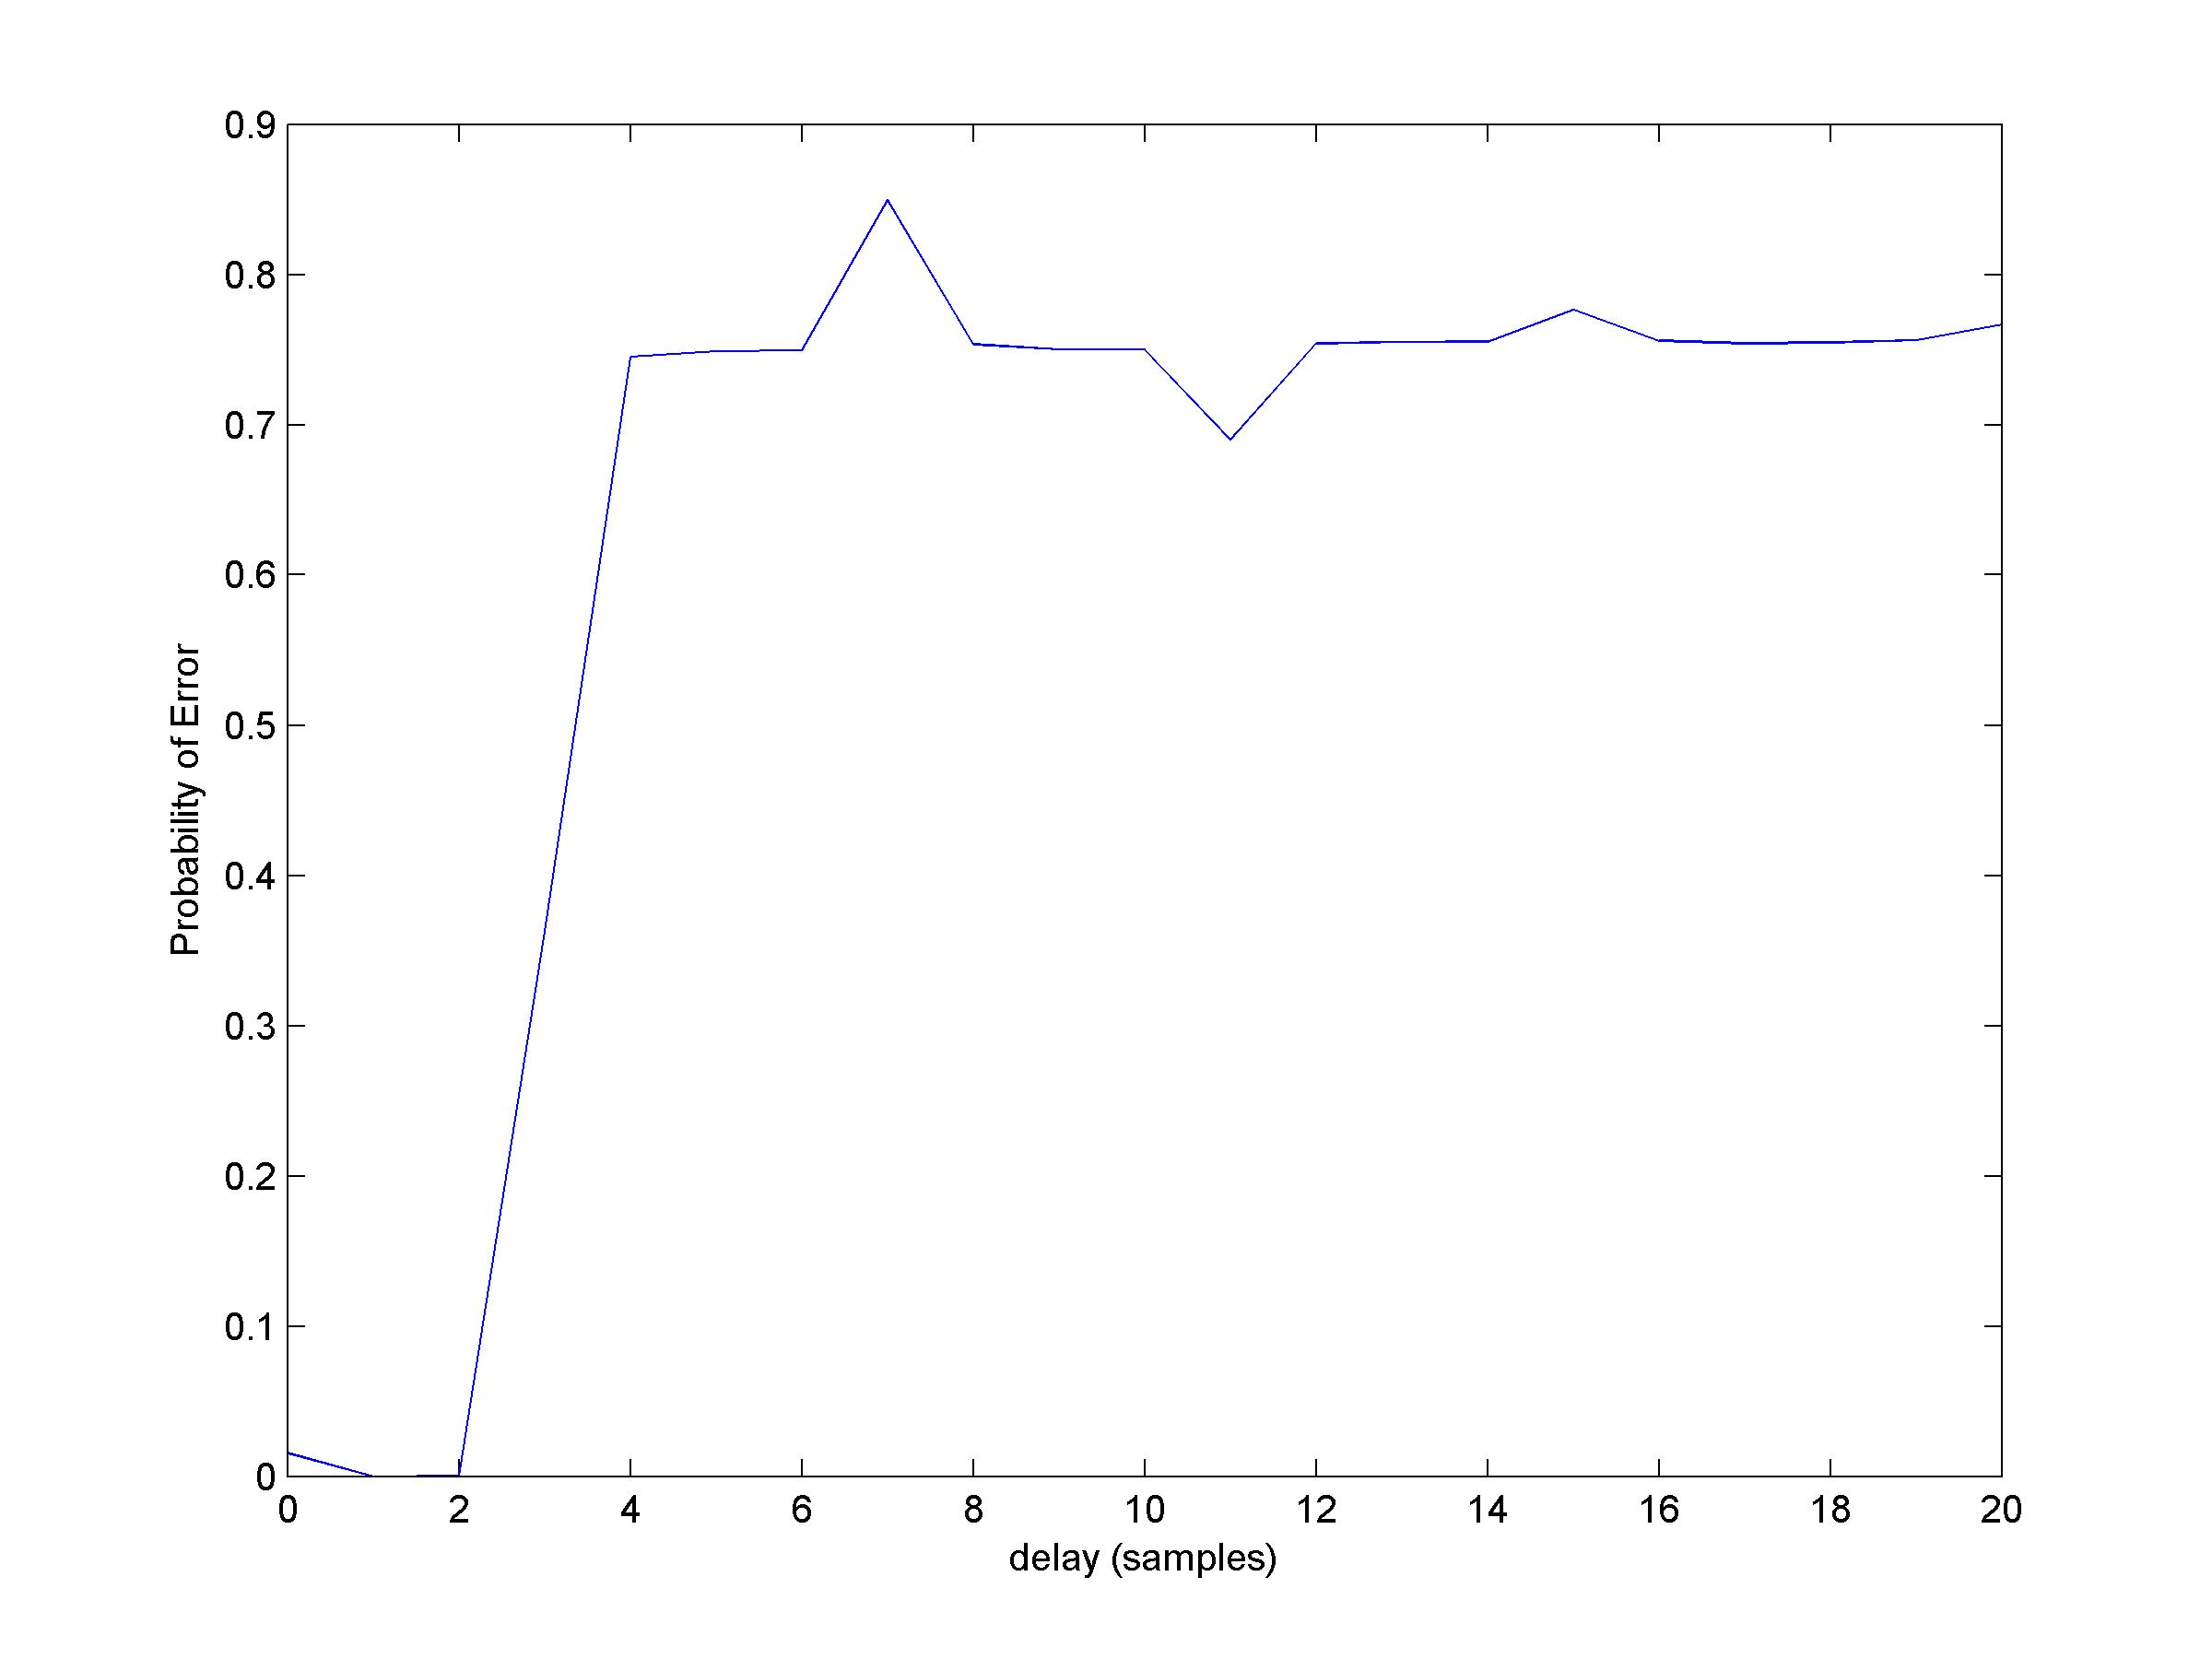
\includegraphics[width=0.6\textwidth]{delaySensitivity.jpg}
\caption{SER plot as a function of delay at the samplin g points of the A/D converter at SNR=20dB (QPSK modulation). \label{fig:delay}}
\end{figure}

\subsection{ZF Equalizer Noise-Enhancement}

A common metric for the price of Zero Forcing is the \emph{noise enhancement}.  Because the equalizer is amplifying the system frequency response in the channel-attenuated zones in order to maintain a uniformly flat character, the noise from the channel gets similarly amplified by the equalizer.  This is the cost of knocking out ISI.  For ZF, this is a factor by which the system SNR must be scaled by in order to maintain equivalent performance after the equalizer as compared to the output after the matched filter in a no-ISI setting.  It can lead to cases where there is large noise PSD compared to the signal after the equalizer.

\subsection{Costas Loop Frequency Offset Tracking}
As explained in Section ~\ref{sec:phaseError} a phase tracker with two integrators are used to cancel out the frequency offset which is introduced to the system in the channel. The problem with using a phase tracker instead of a frequency tracker when there is frequency offset, is that the feedback loop will only get rid of the offset if it is relatively small compared to the sampling period. 

Because both the frequency offset is $100 \mathtt{kHz}$ (period of $10 \mathtt{\mu s}$) and is comparable to our signal bandwidth, and we want our tracking loop settling time to be reasonable, we decided to sample the waveform much faster than necessary in order to have tie resolution to deal with the frequency offset.

\newpage
\section{Results}
\label{sec:results}

\newpage
\section{Conclusion}
\subsection{step 1 conclusion}
This project was a demonstration of a digital communication with various modulation schemes which are:
\begin{itemize}
\item BPSK
\item QPSK
\item 16-QAM
\item 64-QAM
\end{itemize}

Randomly generated and equally probable bits are modulated using the given schemes above.  They are filtered with a square-root raised cosine pulse and passed through an AWGN channel whose noise is varied from tolerable to overpowering.  This can be seen in the both sets of plots.  These plots were made by sending 48,000 bits through the system and measuring the error rate, as explained through the report.

The following are deduced from this step of the project:
\begin{itemize}
\item For each modulation scheme, \emph{increasing} the input SNR \emph{decreases} the probability of symbol error
\item \emph{Increasing} the constellation size \emph{increases} the bit rate.  That being said, the plots show the probability of symbol error \emph{increases} as well.
\item With sufficient simulation test bits, experimental error rates match up with  the theoretical probability of symbol error. 
\item As the constellation size \emph{increases}, the difference between experimental and theoretical bit error rates at low SNR values \emph{amplifies}. However, at high SNR levels, theoretical and experimental bit error rates are almost identical. This is due to the theoretical bit error rates being crudely approximated (dividing the theoretical symbol error rates by the number of bits used per symbol). By doing so, we assume that bit errors are only caused by a one-bit difference.  This underestimates the error rate - simulation symbol errors can occur with more than one bit error. Therefore we see that this approximation works best at high SNR values. 
\item Finally, it must also be mentioned that the theoretical error rates are calculated using Eb/No rather than the symbol SNR. This conversion is made by dividing the SNR by the number of bits used per symbol. Thus, if the theoretical error rates where plotted with Eb/No values as the x-axis the graphs would shift left.  

\end{itemize}


\subsection{step 2 conc}
This section of the project showed off the effects of carrier phase and frequency offsets.  This occurs in real systems when coherency is not maintained.  Synchronization between transmitter and receiver oscillator is not perfectly maintained.  The models showed that symbol error rates remained functional for small errors in phase and frequency.  As phase got to $\frac{\pi}{4}$ off, the constellations became the same as for proper $\frac{\pi}{4}$-QPSK [Section~\ref{sec:qam16_phaseConst}].  At this extreme, there was significant misclassification of symbols.  \\

The frequency errors did completely not ruin the transmissions [\ref{sec:results_fo}].  Because the symbol period was so brief, the accumulation of error for small frequency deviations was kept small.  As the frequency difference climbed, the effect became more and more evident.  The tell-tale sign of an offset in frequency is shown in plots such as Figure~\ref{fig:qpsk_freq}.  The blur along the unit circle demonstrates the frequency error.  The errors were catastrophic in the case of a 10 Hz frequency offset.  \\

From this project, the sensitivity of modulation schemes was analyzed.  Impercise phase and frequency can ruin a data system.  In subsequent phases of the project, remedies for these issues will be explored.



\subsection{Step 3 Conclusion}
\label{sec:conc}

The objective of this step was to recover the system from the phase and frequency offsets that might be present in the received signal. To handle the noncoherent error introduced into the system, feedback loops (Costas and Decision Directed) were installed. These use control feedback to track out the errors by first finding a metric for the error, then using integrators to track away that error. 

The `S' Curve results for the Costas type setup give indication of how the system reacts to different degree phase and frequency error.  Notice, in each of the graphs [~\ref{fig:costasSphase}, \ref{fig:costasSfreq}], the estimation error is periodic.  This is because the the metric does a good job approximating for phase at small phase levels, but of course has some error.  We see the same results in the Decision Directed cases as well [\ref{fig:ddrsphase}, \ref{fig:ddrsfreq}].

In the transience plots, notice that the error in the 6 dB is zero mean and has magnitude around .01.  The 30 dB plot [\ref{fig:costasTransPhase}]  shows the typical convergence shape we would expect.  We feel that the same structure exists in the lower SNR case, but the settling time happens in only a few samples and gets lost.  This pattern is repeated for the frequency estimation trials as well [\ref{fig:costasTransFreq1}, \ref{fig:costasTransFreq2}].  Again, the Decision Directed loops have the same form [\ref{fig:ddrTransphase}, \ref{fig:ddrtransFreq1}, \ref{fig:ddrTransFreq2}].

The constellation plots are also informative.  Note how in the Phase Costas Loop, Figure~\ref{fig:costasConstPhase}, there are a few points that have the stretching characteristic of phase error.  Then the blurring stops and the loop locks on, creating the clumps for the symbols.  This same tracking happens in the Decision Directed constellation [\ref{fig:ddrConstPhase}].  The frequency offsets never show this tracking, perhaps because they get locked on so quickly the tail never appears.

Looking at the loop filter output results for the system where a phase offset is introduced, it can be seen that phase error estimate converges to zero very fast. This means that we don't really need to throw any of the received bits. This result can also be deduced from the BER graphs provided in the results section. When a phase offset is introduced, dropping bits doesn't really change the resulting probability of error of the system. Thus we can conclude that if the phase error estimate converges fast enough dropping bits doesn't really affect the efficiency of the system in term of bit error rate. 

The same results are valid for the system with frequency offset too, as the frequency error estimate reaches the steady-state fast enough that dropping bits doesn't really change the bit error rate of the system. 

\subsection{step 4 conclusion}
The objective of this step was to visualize the effects of data converters in the system model.  Analog and digital waveforms can be safely interchanged only under certain conditions - namely when the sampling is fast enough.  In addition to a minimum sampling rate, low pass filters are necessary to protect against aliasing of high frequency content which should be operated at the linear regions of the $tan(.) $ function due to the bilinear transformation of analog filters into discrete domain.  \\

We included A/D and DAC blocks in our system to see how well the modulation and recovery performed in comparison to earlier trials. The following conclusions are made from the results of this step:

\begin{itemize}
\item The importance of sampling timing on the bit error rate is crucial due to the fact that we using low pass filters at both RX and TX  which delay the signals passing through them. From a sensitivity analysis of the delay through the system, the A/D will sample at varying degrees of synch. From such an experiment written in Appendix~\ref{app:delay}, when all other parameters like SNR and cutoff frequencies are kept equal to the optimal, we end up seeing the system works best at sampling delays 1 and 2. This is shown in Figure~\ref{fig:delay}.
\item A similar analysis is done for the cutoff frequency of the TX reconstruction filter. Recall, this filter is in place to bandlimit the DAC output so the high frequency content in the stairs does not create aliases in the lower, passband. The filter model is controlled by a normalized cutoff frequency, where zero and one are mapped to $\left(0,f_s\right)$.  As such, we expect that the cutoff frequency will not make much difference except if it is lower than $\pi/$(over sampling size of analog signal).  Even by choosing $f_c$ near $\pi/10$ (end of assumed linear region), all frequencies above the sampling frequency will be attenuated and the filter serves its purpose.  However, if $f_c$ gets too low, the information in the waveform may be lost. 
Figure~\ref{fig:freqTX} shows the sensitivity analysis of the anti-aliasing LPF normalized cutoff frequency.  The graph confirms the expected behavior discussed above.
\item We performed an equivalent analysis on the cutoff frequency in the RX noise-limiting filter.  This filter was aimed to low pass filter the high frequency content from the noise and only allow the signal through.  The same filter model was used with a lower cut-off frequency, so a similar trend was expected. Again at near zero cutoff, again we expect loss of data. But also this time, when the cut-off frequency is increased to the limits of the linear region we see an increase of the BER due to the fact that more noise is passing through the filter. Figure~\ref{fig:freqRX} shows the sensitivity analysis of the noise-limiting LPF normalized cutoff frequency.  The graph confirms the expected behavior discussed above.
\end{itemize}

In conclusion we have seen that the system works best at the following:
\begin{itemize}
\item RX and TX filters  at $w_c$ which are in the range $\left[0.02,0.09\right]  $
\item Sampling points at a delay of 1 sample.
\end{itemize}

Although the results obtained in this step are close to the theoretical values, they can never achieve the theoretical limit due to the fact that we need infinite over sampling to construct an analog signal from a digital signal. Thus the theoretical limits form a lower bound to a system with data converters. 

\section{Future Work}

\appendix
\newpage
\bibliographystyle{plain}
\bibliography{final}
\newpage
%% the \\ insures the section title is centered below the phrase: Appendix B
%\section{Project Assignment}
%\label{app:assign}
%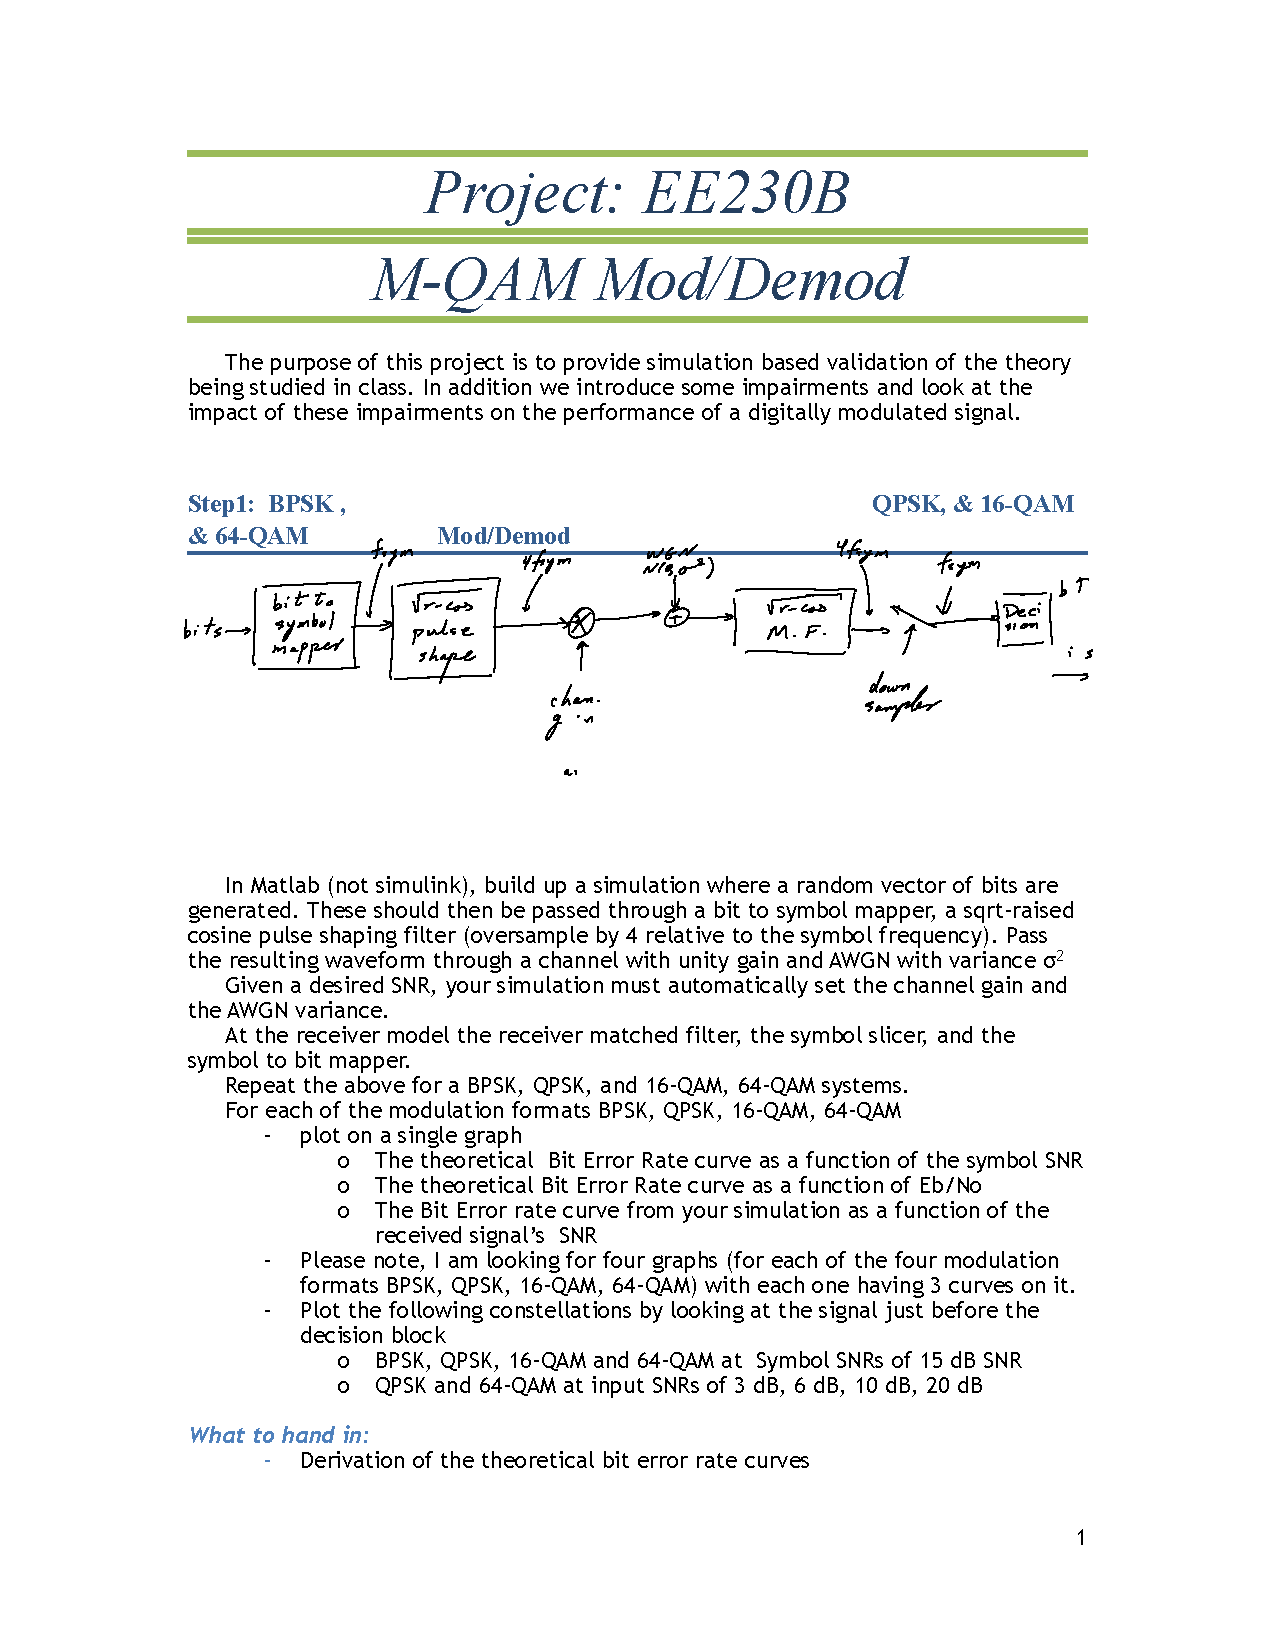
\includepdf[pages={1-5}]{project_overview.pdf}
%\cleardoublepage
%\newpage

\section{Communication Background}

\subsection{Feedback Theory}
\label{sec:feedback}
In control theory when there is steady state error in the open loop system, feedback, or `closing the loop' can track out the error. This is just the case because of the frequency error steady state error.  Depending on the order of the system, this error can become unbounded and damning.  Simple feedback can track this error if the open loop system Type is 0.  \footnote{Recall, a system is of Type N when there are N poles at the s-plane origin.}  Here however, we have a Type 1 system - ramp input of phase error.  An additional integrator increases the order of the closed loop system to allow bounding of higher type systems. Notice in Figure~\ref{fig:costas}, the loop filter is Proportional-Integral.  With two integrators in the feedback path, we can bound phase error to a constant steady state level.  Because frequency can be thought of as first order phase [\ref{eq:phaseFreq}], we track out the frequency error.\\

\subsection{Data Conversion}
\label{sec:converter}
This step of the project introduces complications from using computers and digital methods to analyze analog signals.  Data conversion, the process of taking a continuous signal and descretizing it, can lead to additional and sometimes catastrophic errors.\\

Recall, digital signals are quantized into samples, discrete points in time.  Conversely, an analog signal has a continuous value.  Going from one to the other requires a converter.  To take an analog signal and digitize it, an Analog-to-Digial Converter (A/D) is used.  Both types of signals are shown in Figure~\ref{fig:digitization}.  There is a wrinkle: the rate of conversion is critical to preserving the information.  By the Nyquist-Shannon Sampling Theorem (\ref{eq:nyquist}), the sampling frequency must be at least twice the highest frequency in the signal.  Without reaching this frequency, the samples can wrongfully convey a lower frequency signal, alias, of the true signal.  This is shown in Figure~\ref{fig:alias}.  

\begin{align}
\label{eq:nyquist}
f_s \geq 2 f_{max}
\end{align}

\begin{figure}[h]
        \centering
        \begin{subfigure}[b]{0.4\textwidth}
                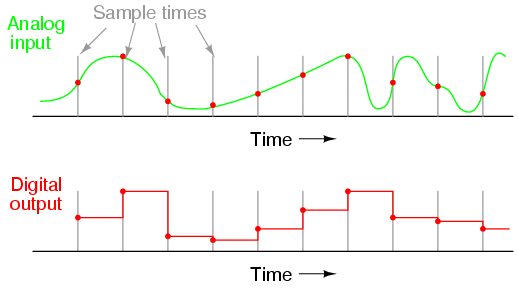
\includegraphics[width=\textwidth]{digitization.png}
                \caption{Analog and Digital signals}
                \label{fig:digitization}
        \end{subfigure}%
        \qquad \quad %add desired spacing between images, e. g. ~, \quad, \qquad etc.
          %(or a blank line to force the subfigure onto a new line)
        \begin{subfigure}[b]{0.5\textwidth}
                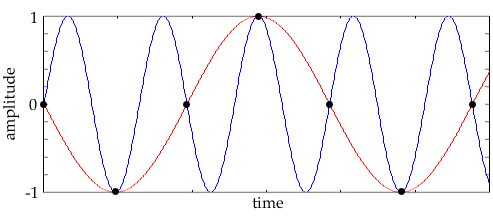
\includegraphics[width=\textwidth]{aliasing.jpg}
                \caption{Aliasing \label{fig:alias}}
                \label{fig:alias}
        \end{subfigure}
        \caption{Digital Conversion \label{fig:digitize}}
\end{figure}

\newpage
\subsection{Inter Symbol Interference and Equalization}
\label{sec:ISIbackground}
Inter Symbol Interference (ISI) is when residual signal from symbols meddles the level of subsequent symbols.  Because of the bandlimiting, where the response of the system is 0 above a limiting frequency, the symbols will interfere with one another. To deal with the dispersion, the Zero-ISI condition [\ref{thm:zero}] must be met.  A number of techniques can be utilized to accomplish what effectively amounts to canceling out delayed versions of symbols:

\begin{itemize}
\item Use $C^{-1}\left(f\right)$ to undo the channel
\item Use precoding
\item Use Nyquist's Pulse-Shaping Criterion and MLSE
\item Use an Equalizer
\end{itemize}
For this to be effective, the system channel medium must be known or estimated [Section~\ref{sec:estimate}].\\

\begin{figure}[b]
\centering
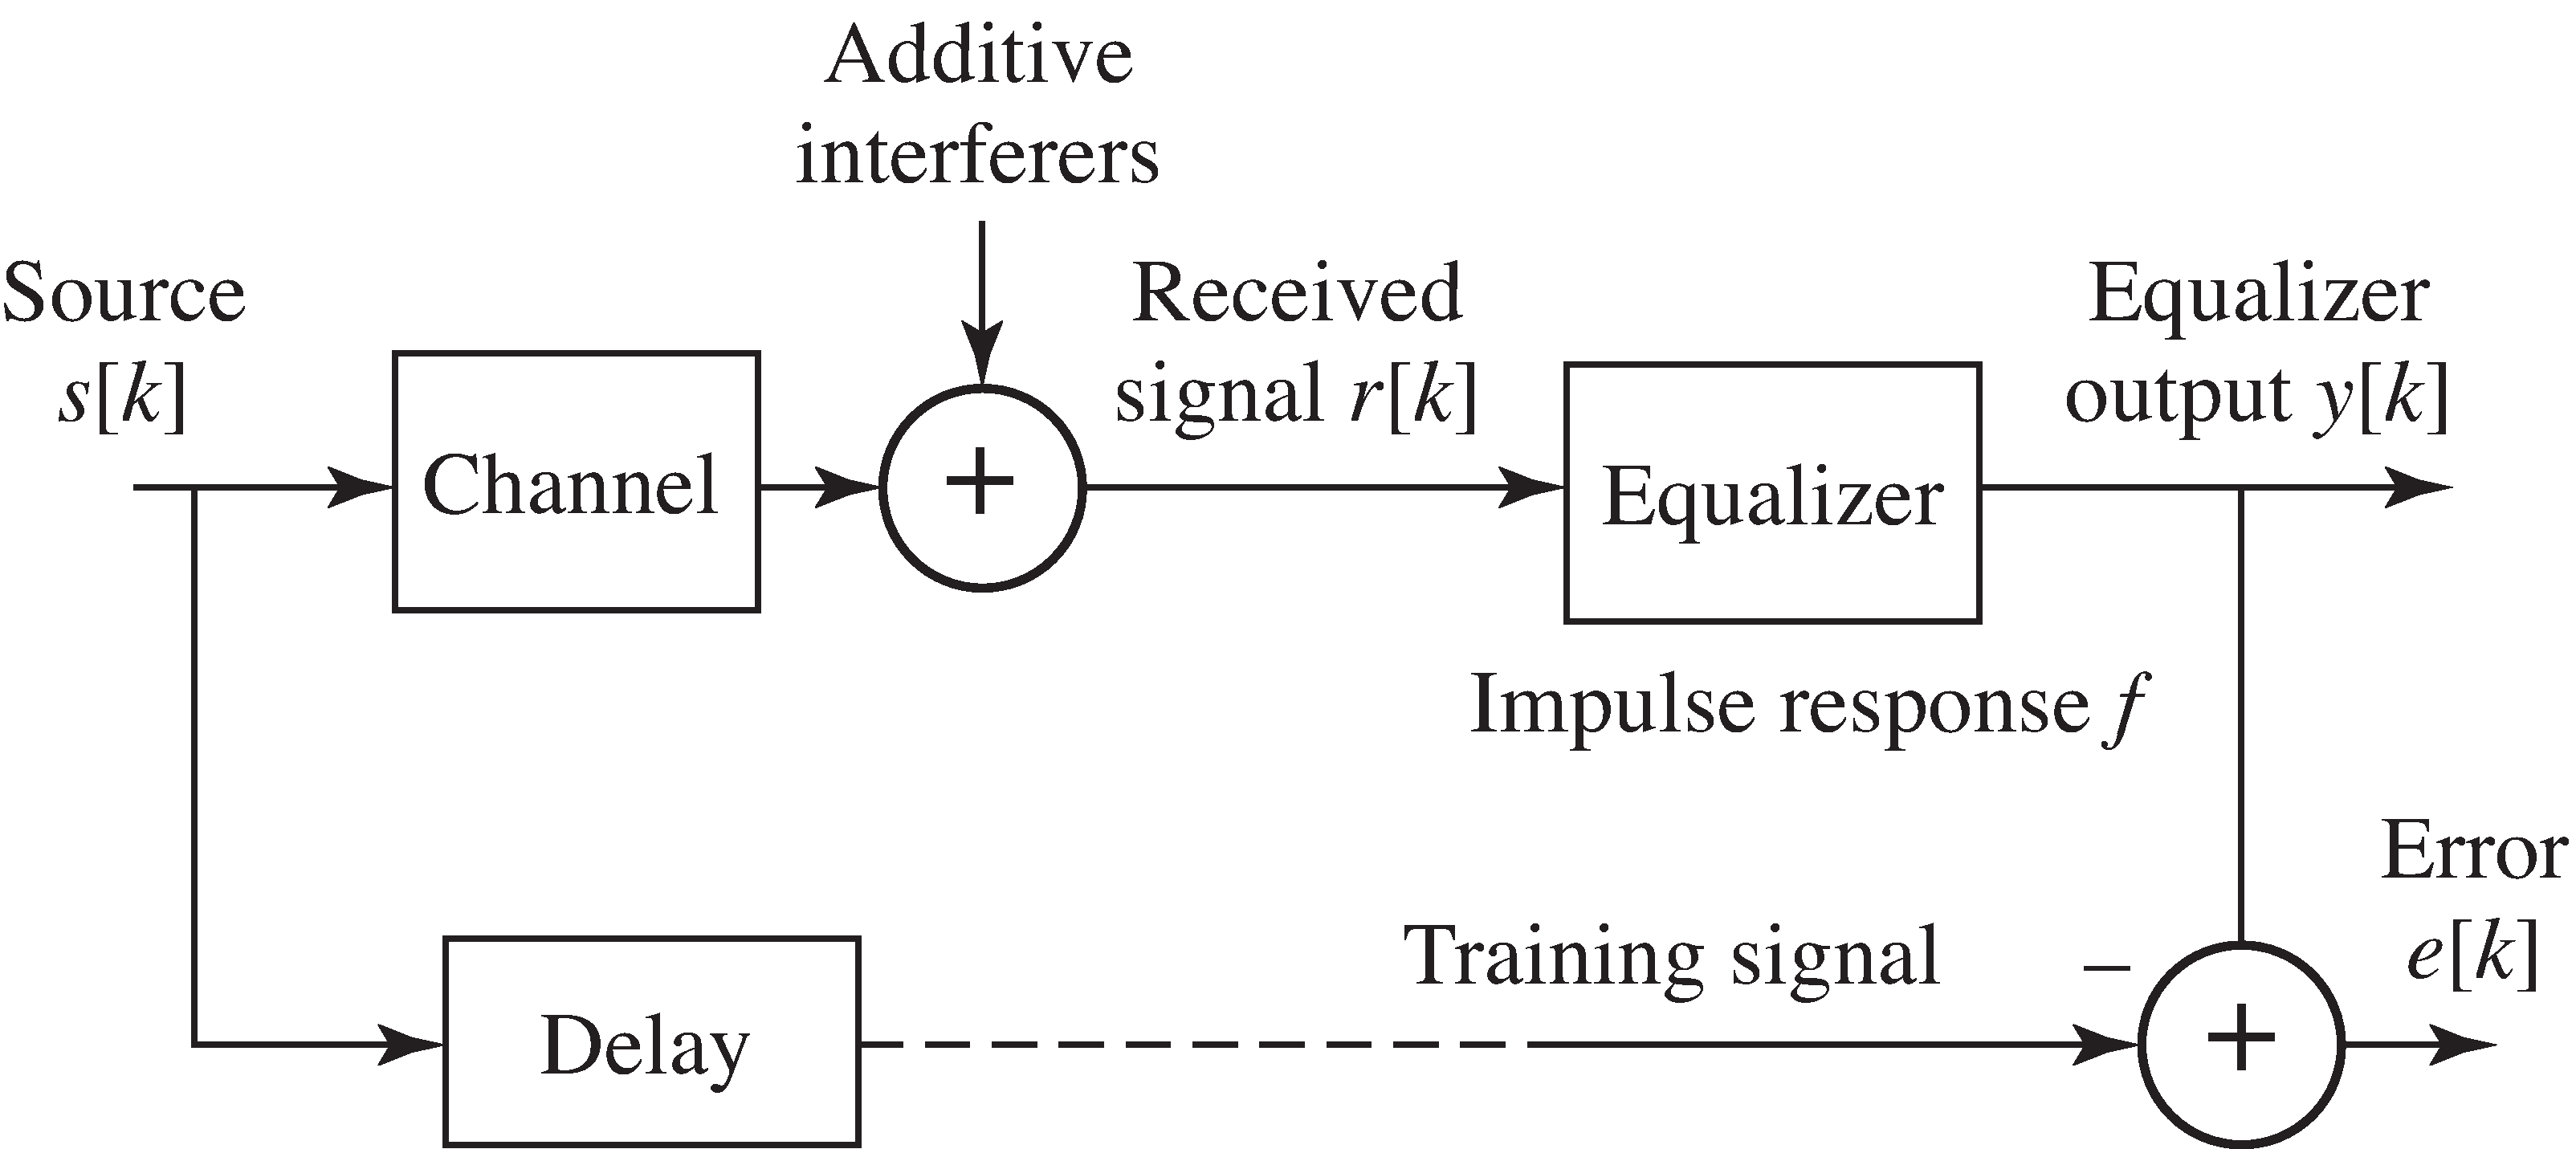
\includegraphics[width=.6\textwidth]{equalizer.png}
\caption{Generic Equalizer Filter to zero out the ISI\label{fig:equalizer}}
\end{figure}

\begin{thm}
\label{thm:zero}
Zero-ISI:
$$x\left(nT\right) = \left\{
\begin{array}{c c}
1 & \quad n=0 \\
0 & \quad \text{else}
\end{array} \right.$$
\end{thm}

\subsection{Estimation}
\label{sec:estimate}
Considering this system, where Table~\ref{tab:filtersummary} describes the variables and Table~\ref{tab:Paramsummary} describes the dimension parameters, the channel is must be known before anything else. \\

To do channel estimation, a known sequence is sent through the system and error on the signal at output is measured.  That is, the input ($r$) and output ($y$) of the filter are known, and the tap weights ($f$) are to be determined - we can look at the impulse response of the unknown channel facing the known input.  Once the channel is understood, we can use an assortment of metrics to perform equalization.

\subsection{Equalization}
\label{sec:equal}
An equalizer is a filter that zeros out the ISI in the end-to-end system.  It can be preset to handle the channel, or can adapt to the time-varying nature of a channel.  In the latter case, the equalizer parameter are adjusted on the fly by periodic transmission of a known sequence to re-estimate the channel.  In either case, the equalizer is a filter whose frequency response counteracts the system model such that Condition~\ref{thm:zero} is met. 

\begin{table}[H]
\begin{center}
\begin{tabular}{|c|c|c|c|}
\hline Variable & Meaning & Dimensions \\
\hline \hline
$\mathbf{I}$ & Symbol Source & $ m \times 1$ \\ \hline
$\mathbf{s}$ & Source & $m\times 1 $\\ \hline
$\mathbf{r}$ & Received Signal & $m\times 1$ \\ \hline
$R$ & Channel Response Matrix & $p\times n$ \\ \hline
$\mathbf{f}$ & Tap Line / Impulse Response & $n\times 1 $ \\ \hline
$\mathbf{y}$ & Equalizer Output & $ m\times 1 $ \\ \hline
 $\mathbf{e}$ & Training Error & $ m\times 1 $ \\ \hline
\end{tabular}
\caption{Summary of Signal Variables} \label{tab:filtersummary}
\end{center}
\end{table}

\begin{table}[b]
\begin{center}
\begin{tabular}{|c|c|}
\hline Parameter & Meaning \\
\hline \hline
$m$ & Signal Length \\ \hline
$N$ & Channel Filter Order \\ \hline
$n$ & Equalizer Filter Order \\ \hline
$p$ & Training Sequence Length \\ \hline
\end{tabular}
\caption{Summary of Parameters} \label{tab:Paramsummary}
\end{center}
\end{table}

The FIR form of the equalizer can then be written as Equation~\ref{eq:equalizerVector} and Equation~\ref{eq:equalizerMatrix}.  The compact form of this relation uses a matrix equation where the filter is expressed as a Toeplitz matrix.  This neat fact allows us to use the power of linear algebra to solve for the zero forcing channel.  
  
 
\begin{figure}[H]
\centering
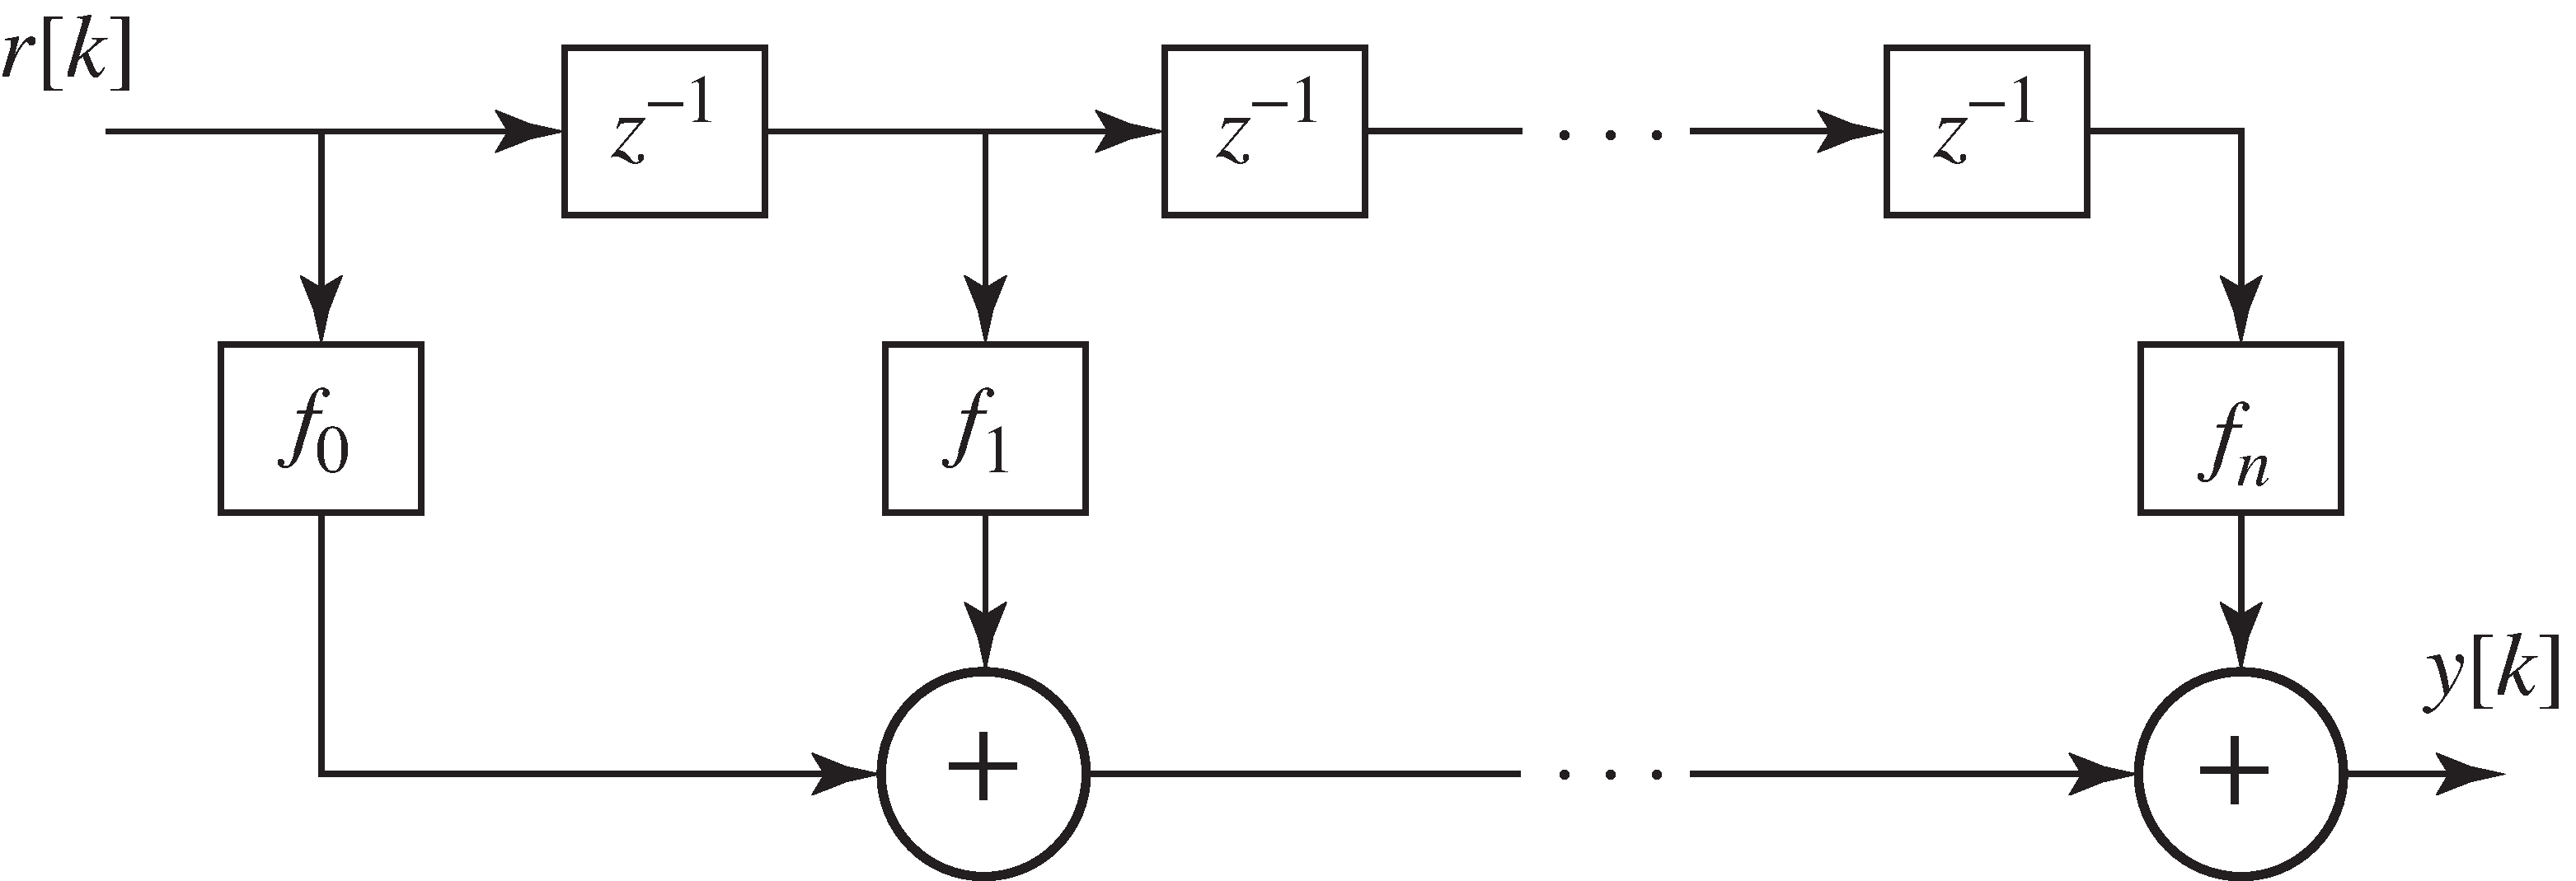
\includegraphics[width=.6\textwidth]{tapEqualizer.png}
\caption{Tapped Delay Line Represenation\label{fig:tap}}
\end{figure}

\begin{equation}
\label{eq:equalizer}
y\left[k\right] = \sum_{j=0}^n f_jr\left[k-j\right]
\end{equation}

The direct form of the FIR equalizor is shown in Figure~\ref{fig:tap}.  This is a subblock diagram view of the equalizer filter.  The transfer function can be gathered from Equation~\ref{eq:equalizer}.  The objective of this filter is to counter the system channel.  \\

\begin{equation}
\label{eq:equalizerVector}
\left[ \begin{array}{c}
 y \left[n+1\right] \\
 y \left[n+2\right] \\
 y \left[n+3\right] \\
\vdots  \\
y\left[ p \right] \end{array} \right] = 
\begin{bmatrix} 
r \left[ n+1\right]  & r[n] & \cdots & r\left[ 1 \right] \\ 
r \left[ n+2\right]  & r[n+1] & \cdots & r\left[ 2 \right] \\ 
r \left[ n+2\right]  & r[n+2] & \cdots & r\left[ 3 \right] \\ 
\vdots & \vdots & & \vdots \\
r \left[p \right] & r\left[ p-1 \right] & \cdots & r\left[ p-n \right]
\end{bmatrix}
 \left[ \begin{array}{c} f_0 \\ f_1 \\ f_2 \\ \vdots \\ f_n \end{array} \right]
\end{equation}

\begin{equation}
\label{eq:equalizerMatrix}
\mathbf{y} = R\mathbf{f}
\end{equation}
What we want is force the channel to zero for all other symbols other than the present one.  As an aside, because there is delay in the system, the intuitive sense of causality is blurred. That is, forward symbols from the present moment can actually cause interference to the present symbol. 

\section{Random Bit Sequence Generator}
\label{app:random_bit_generator}
\lstinputlisting{random_bit_generator.m}

\section{Bit to Symbol Mapper}
\label{app:bittosym}

\subsection{QPSK Modulation}
\label{app:qpsk_mod}
\lstinputlisting{qpsk_mod.m}

\subsection{16-QAM Modulation}
\label{app:qam_16_mod}
\lstinputlisting{QAM_16_mod.m}

\section{Up Sampler}
\label{app:impulse_train}
\lstinputlisting{impulse_train.m}

\section{Square Root Raised Cosine Filter}
\label{app:sqrt_raised_cosine}
\lstinputlisting{sqrt_raised_cosine.m}

\section{Channel Models}
\subsection{Bandlimited Channel}
\label{app:bandlimited}
\lstinputlisting{bandlimited_channel.m}

\subsection{Ideal Complex AWGN Channel}
\label{app:awgn_channel}
\lstinputlisting{awgn_complex_channel.m}

\subsection{Frequency Offset}
\label{app:freq}
\lstinputlisting{freq_offset.m}

\section{Sampler}
\label{app:sampler}
\lstinputlisting{sampler.m}

\section{Decision Block}
\label{app:dblocks}
\subsection{QPSK Demodulation}
\label{app:qpsk_demod}
\lstinputlisting{qpsk_demod.m}

\subsection{16-QAM Demodulation}
\label{app:16qam_demod}
\lstinputlisting{QAM_16_demod.m}

\section{Equalizers}
\subsection{ZF Equalizer}
\lstinputlisting{ZFEqualizer.m}


\section{Butterworth Filter}
\label{app:butterworth}
\lstinputlisting{ButterworthFilter.m}

\section{Conversion}
\label{app:convert}
\subsection{Analog-to-Digital Converter}
\label{app:ad}
\lstinputlisting{AD_conv.m}
\subsection{Digital-to-Analog Converter}
\label{app:da}
\lstinputlisting{DA_conv.m}

\subsection{Zero Hold}
\label{app:zero}
\subsection{Decimation}
\lstinputlisting{ZeroHoldDecimation.m}
\subsection{Interpolation}
\lstinputlisting{ZeroHoldInterpolation.m}


\section{Simulations}
\subsection{QPSK Simulation}
\lstinputlisting{final_sim_qpsk.m}

\subsection{16-QAM Simulation}
\lstinputlisting{final_sim_QAM16.m}

\end{document}
